% ==============================================================================
% ================================= Aufgabe 5 =================================
% ==============================================================================

\chapter{Simulationsexperimente und Auswertung \textit{5}}
\label{chap:aufgabe5}
\thispagestyle{fancy}

% ==============================================================================
% ============== Aufgabe 5A - Leistungskennzahlen der Simulation ==============
% ==============================================================================

\section{Leistungskennzahlen der Simulation \textit{5a}}
\label{sec:aufgabe5a}

\subsection{Aufgabenstellung}

Lassen Sie nun die vollständige Simulation laufen: Nutzen Sie mindestens eine Karte, und simulieren Sie Varianten mit 3, 5 und 10 Agenten unterschiedlicher Typen (Standard und Express). Nun müssen die Agenten und Ihre Software tatsächlich vollständig funktionieren, das heißt Pakete erzeugen, das Bieterverfahren durchführen; die Agenten müssen Pakete aufnehmen und abliefern. Messen Sie dafür die Leistungskennzahlen des Systems: durchschnittliche Lieferzeit vom Erzeugen bis zur Zustellung eines Pakets, die Erfolgsquote (prozentualer Anteil der Aufträge, die innerhalb der vorgegebenen Maximalzeit erledigt werden) und die durchschnittliche Pfadlänge pro Auftrag und Agent.

\subsection{Theoretische Grundlagen}

Für die Leistungsbewertung des Multiagentensystems werden drei Kennzahlen verwendet, die die wesentlichen Zielgrößen eines verteilten Liefersystems abdecken: \textit{Durchlaufzeit} (Zeit vom Auftragseingang bis zur Auslieferung), \textit{Servicegrad} (Anteil der fristgerecht erfüllten Aufträge) und \textit{Wegaufwand} pro Auftrag. Diese drei Größen erfassen die Zielkriterien Geschwindigkeit, Zuverlässigkeit und Effizienz und sind daher für die vergleichende Auswertung verschiedener Agentenkonfigurationen geeignet.

Die Experimente folgen dem Vorgehen der \textit{vergleichenden Simulation}: Pro Agentenkonfiguration werden mehrere unabhängige Läufe mit unterschiedlichen Zufalls-Seeds durchgeführt, um statistische Robustheit zu erreichen. Die Ergebnisse werden als Mittelwerte mit Standardabweichung über die Läufe berichtet.

Eine zentrale Voraussetzung für aussagekräftige Messungen ist, dass die Agenten über die vollständige Simulationsdauer aktiv bleiben. Die Batteriekapazität aus Aufgabe~1b (100 bzw.\ 120 Einheiten) war auf kurze Läufe ausgelegt; bei der für 5a erforderlichen Simulationstiefe von 200 Schritten erschöpften alle Agenten ihre Batterie nach etwa 100 Schritten, sodass die zweite Hälfte der Läufe ohne Agentenaktivität verlief. Um dies zu beheben, wurden die Batteriekapazitäten erhöht und eine \textit{Batterie-Regeneration im Idle-Zustand} eingeführt.

\subsection{Implementierung}

Aufgabe~5a führt das neue Modul \texttt{experiment.py} ein, das die Simulationsläufe, Metriken-Aggregation, CSV-Ausgabe und Plot-Erzeugung kapselt. Die drei bestehenden Module \texttt{package.py}, \texttt{agent.py} und \texttt{simulation.py} werden um Metriken-Tracking und einen Headless-Modus erweitert.

\paragraph{Design-Entscheidung: Eigenes Modul \texttt{experiment.py}.}
Die Experiment-Logik wird bewusst nicht in \texttt{main.py} integriert. Der Orchestrator startet weiterhin die interaktive Simulation mit \acs{GUI}; die Auswertung ist ein separater Anwendungsfall ohne grafische Ausgabe. Diese Trennung folgt dem bereits etablierten Prinzip: \texttt{main.py} bleibt ein reiner Starter, die Experimente sind ein eigenständiger Einstiegspunkt.

\paragraph{Design-Entscheidung: Headless-Modus über Config-Flag.}
Die Simulation erhält einen \texttt{verbose}-Parameter. Im Headless-Modus (\texttt{verbose=False}) werden alle \texttt{print}-Aufrufe in \texttt{\_log\_step} übersprungen, während die fachliche Logik unverändert bleibt. Der \texttt{subprocess}-Aufruf für \acs{PROLOG}-Abfragen ist davon nicht betroffen -- der Vorfilter aus Aufgabe~4c bleibt auch im Experiment aktiv.

% ======= config.py – Block 5A und Refactorings =======

\subsubsection{Konfiguration \texttt{config.py} – Parameter und Refactorings}

Der neue Konfigurationsblock definiert alle experiment-spezifischen Werte. Zusätzlich wurden die Batteriewerte aus Aufgabe~1b sowie die Paketparameter aus Aufgabe~2b an die Anforderungen der Experimente angepasst.

\paragraph{Refactoring 1B – Batteriekapazität.}
Die Batteriewerte aus Aufgabe~1b wurden von 100 auf 300 (Standard) bzw.\ von 120 auf 400 (Express) erhöht:

\lstinputlisting[
    language=python,
    style=python,
    caption={Erhöhte Batteriekapazität (\texttt{config.py})},
    label={lst:config_5a_battery},
    firstline=160,
    lastline=162
]{asset/code/5A-config.py}

\textbf{Begründung:} Bei 200 Simulationsschritten und einem Basisverbrauch von 1 Einheit pro Schritt (plus Cargo) reichte die ursprüngliche Kapazität nur für die halbe Simulationsdauer. Die Erhöhung ist keine willkürliche Verstärkung, sondern eine realistische Anpassung an die tatsächliche Einsatzdauer -- vergleichbar mit einem längeren Akku für einen längeren Arbeitstag. Die historische 1b-Dokumentation bleibt unverändert (Schichtungsprinzip).

\paragraph{Refactoring 2B – Deadline und Paketintervall.}
Die Deadline für Pakete wurde von 15 auf 100 Schritte erhöht, das Paketgenerierungs-Intervall von 5 auf 10 Schritte:

\lstinputlisting[
    language=python,
    style=python,
    caption={Angepasste Paketparameter (\texttt{config.py})},
    label={lst:config_5a_deadline},
    firstline=264,
    lastline=266
]{asset/code/5A-config.py}

\textbf{Begründung Deadline:} Die ursprüngliche Deadline von 15 Schritten war nie bindend, weil sich die Agenten vor Aufgabe~3c zufällig bewegten. Mit der Einführung der Wegplanung in 3c wurde die zu knappe Deadline erstmals wirksam -- die typischen Lieferzeiten lagen bei 30--60 Schritten, sodass die Mehrheit der Aufträge bereits vor der Zustellung verfiel. Mit der neuen Deadline von 100 Schritten erhalten Standard-Agenten ausreichend Zeit, auch weitere Wege zu absolvieren.

\textbf{Begründung Intervall:} Das Intervall von 5 Schritten erzeugte 40 Pakete in 200 Schritten, mit nur 3 Agenten war dies eine Überlast, die zu häufigen Deadlocks in Korridoren führte. Das neue Intervall von 10 Schritten erzeugt 20 Pakete -- ausreichend für statistische Aussagen, aber ohne das System zu überlasten.

\paragraph{Neuer Block 5A – Experiment-Parameter.}
Der neue Block umfasst alle Steuerungswerte für die Experimente:

\lstinputlisting[
    language=python,
    style=python,
    caption={5A-Konfiguration (\texttt{config.py})},
    label={lst:config_5a},
    firstline=422,
    lastline=496
]{asset/code/5A-config.py}

Die Konfiguration umfasst sechs Kategorien:
\begin{itemize}
    \item \textbf{Experimente} -- Anzahl der Runs pro Konfiguration (5), Simulationsschritte pro Run (200), Start-Seed (42), Batterie-Regeneration pro Idle-Schritt (2), Verbose-Flags für Produktiv- und Experiment-Modus.
    \item \textbf{Agenten-Konfigurationen} -- drei Konfigurationen als Liste von Dicts; die Zuordnung $\{$\texttt{TypeStandard}$:$ Anzahl, \texttt{TypeExpress}$:$ Anzahl$\}$ ist selbstdokumentierend.
    \item \textbf{Ergebnis-Pfade} -- CSV-Ziel und drei PNG-Pfade.
    \item \textbf{Statistics-Keys} -- Schlüssel für das Metriken-Dictionary, inkl.\ Standardabweichungs-Schlüssel.
    \item \textbf{CSV} -- Header-Zeile, Spalten-Schlüssel und Trennzeichen (\texttt{;}, weil Excel mit deutschem Locale sonst alle Werte in eine Spalte schreibt).
    \item \textbf{Plots} -- Backend (\texttt{Agg} für Headless), Farbe, Breite, Fehlerbalken-Style, Titel, Achsen-Beschriftungen.
    \item \textbf{Logging} -- Templates für Run-Header, Aggregations-Tabelle und Speicher-Bestätigungen.
\end{itemize}

Die Validierungsliste in \texttt{validate\_config()} wird um alle neuen Konstanten erweitert (vgl. Abschnitt~\ref{sssec:config_validierung}).

% ======= package.py – Metriken-Felder =======

\subsubsection{Modul \texttt{package.py} – Metriken-Felder}

Der Import wird um die beiden neuen Status-Werte erweitert:

\lstinputlisting[
    language=python,
    style=python,
    caption={Erweiterte Imports (\texttt{package.py})},
    label={lst:package_imports_5a},
    firstline=13,
    lastline=14
]{asset/code/5A-package.py}

Der Konstruktor der \texttt{Package}-Klasse wird um drei Felder erweitert, die für die Leistungsmessung benötigt werden:

\lstinputlisting[
    language=python,
    style=python,
    caption={Neue Metriken-Felder im Konstruktor (\texttt{package.py})},
    label={lst:package_ctor_5a},
    firstline=34,
    lastline=36
]{asset/code/5A-package.py}

\begin{itemize}
    \item \texttt{delivered\_step} -- der Step, in dem das Paket zugestellt wurde.
    \item \texttt{expired\_step} -- der Step, in dem die Deadline überschritten wurde.
    \item \texttt{delivery\_path\_length} -- die Pfadlänge des liefernden Agenten, festgehalten zum Zeitpunkt der Zustellung.
\end{itemize}

Zwei neue Methoden markieren die Zustandsübergänge:

\lstinputlisting[
    language=python,
    style=python,
    caption={Neue Methoden \texttt{mark\_delivered}, \texttt{mark\_expired} (\texttt{package.py})},
    label={lst:package_methods_5a},
    firstline=47,
    lastline=55
]{asset/code/5A-package.py}

\texttt{mark\_delivered(step, path\_length)} erhält die Pfadlänge des liefernden Agenten als zweiten Parameter. Dadurch wird die Pfadlänge \textit{pro zugestelltem Paket} erfasst, nicht pro Agent über die Gesamtlaufzeit -- nur so ist die Metrik „durchschnittliche Pfadlänge pro Auftrag und Agent" aussagekräftig.

% ======= agent.py – Pfadlängen-Tracking =======

\subsubsection{Modul \texttt{agent.py} – Pfadlängen-Tracking und Kollisionsprüfung}

Der Konstruktor der \texttt{Agent}-Klasse erhält zwei neue Felder zur Pfadlängen-Messung:

\lstinputlisting[
    language=python,
    style=python,
    caption={Neue Pfadlängen-Felder im Konstruktor (\texttt{agent.py})},
    label={lst:agent_ctor_5a},
    firstline=110,
    lastline=111
]{asset/code/5A-agent.py}

Die Methode \texttt{try\_move} wird um zwei Aspekte erweitert: eine Prüfung auf belegte Zielzellen durch andere Agenten und die Inkrementierung der Pfadlängen:

\lstinputlisting[
    language=python,
    style=python,
    caption={Erweiterte \texttt{try\_move} (\texttt{agent.py})},
    label={lst:agent_trymove_5a},
    firstline=131,
    lastline=143
]{asset/code/5A-agent.py}

\textbf{Warum die Kollisionsprüfung?} In Aufgabe~1c wurde eine Kollisionsauflösung ausschließlich nachträglich in \texttt{Simulation.\_resolve\_collisions} durchgeführt -- Agenten durften auf dieselbe Zelle ziehen und wurden danach zurückgesetzt. Für die Experimente erwies sich dies als ungeeignet: In engen Korridoren pendelten zwei Agenten endlos zwischen ihren Vorpositionen, ohne die Korridore zu passieren. Die Prüfung in \texttt{try\_move} verhindert den Zug auf belegte Zellen von vornherein. Die Simulation bleibt robust -- die \texttt{\_resolve\_collisions}-Logik aus 1c bleibt als Sicherheitsnetz erhalten, wird aber im Normalfall nicht mehr ausgelöst.

Zusätzlich wurde in \texttt{decide\_action} eine Schutzprüfung eingebaut, die einen IndexError verhindert, wenn die \acs{Astern}-Route nur aus der aktuellen Position besteht (Start~$=$~Ziel):

\lstinputlisting[
    language=python,
    style=python,
    caption={Schutzprüfung in \texttt{decide\_action} (\texttt{agent.py})},
    label={lst:agent_decide_5a},
    firstline=165,
    lastline=166
]{asset/code/5A-agent.py}

Die Methode \texttt{deliver} übergibt die Pfadlänge an die Paket-Markierung:

\lstinputlisting[
    language=python,
    style=python,
    caption={Erweiterte \texttt{deliver} (\texttt{agent.py})},
    label={lst:agent_deliver_5a},
    firstline=190,
    lastline=190
]{asset/code/5A-agent.py}

Die Pfadlängen werden inkrementiert, sobald ein Zug tatsächlich erfolgreich war. \texttt{path\_length\_current\_task} wird beim Start eines neuen Tasks in \texttt{\_try\_start\_next\_task} auf 0 zurückgesetzt:

\lstinputlisting[
    language=python,
    style=python,
    caption={Reset der Aufgaben-Pfadlänge (\texttt{agent.py})},
    label={lst:agent_reset_5a},
    firstline=237,
    lastline=237
]{asset/code/5A-agent.py}

Und in \texttt{\_replan} wird das erneute Loggen einer unveränderten Route unterdrückt -- dies verhindert die Log-Flut, die bei dauerhaft blockierten Routen entstand:

\lstinputlisting[
    language=python,
    style=python,
    caption={Log-Unterdrückung bei unveränderter Route (\texttt{agent.py})},
    label={lst:agent_replan_5a},
    firstline=265,
    lastline=266
]{asset/code/5A-agent.py}

% ======= agent.py – create_agents parametrisierbar =======

\subsubsection{Modul \texttt{agent.py} – Parametrisierbare Agenten-Fabrik}

Die Funktion \texttt{create\_agents} erhält drei neue Parameter mit Config-Defaults, damit dieselbe Funktion sowohl von \texttt{main.py} (mit den 1b-Standardwerten) als auch von \texttt{experiment.py} (mit den konfigurationsspezifischen Werten) verwendet werden kann:

\lstinputlisting[
    language=python,
    style=python,
    caption={Parametrisierte Agenten-Fabrik (\texttt{agent.py})},
    label={lst:agent_factory_5a},
    firstline=318,
    lastline=338
]{asset/code/5A-agent.py}

Die bestehenden Aufrufe in \texttt{main.py} bleiben unverändert -- die Default-Werte greifen und entsprechen dem bisherigen Verhalten.

% ======= simulation.py – verbose, BatteryRegen, Deadline-Check, Statistik =======

\subsubsection{Modul \texttt{simulation.py} – Headless-Modus, Batterie-Regeneration, Deadline-Prüfung und Metriken}

Die Imports werden um die neuen 5A-Konstanten und der 2B-Status-Werte erweitert:

\lstinputlisting[
    language=python,
    style=python,
    caption={Erweiterte Imports (\texttt{simulation.py})},
    label={lst:sim_imports_5a},
    firstline=38,
    lastline=50
]{asset/code/5A-simulation.py}

Der Konstruktor erhält einen \texttt{verbose}-Parameter (Default aus Config):

\lstinputlisting[
    language=python,
    style=python,
    caption={Erweiterter Konstruktor (\texttt{simulation.py})},
    label={lst:sim_ctor_5a},
    firstline=59,
    lastline=61
]{asset/code/5A-simulation.py}

Der \texttt{\_log\_step}-Methode wird ein Guard vorangestellt, der im Headless-Modus alle Ausgaben unterdrückt:

\lstinputlisting[
    language=python,
    style=python,
    caption={Verbose-Guard im Step-Logging (\texttt{simulation.py})},
    label={lst:sim_log_5a},
    firstline=121,
    lastline=121
]{asset/code/5A-simulation.py}

Die \texttt{\_agent\_step}-Methode wird um die Batterie-Regeneration im Idle-Zustand und um die Weitergabe der Simulation an \texttt{try\_move} erweitert:

\lstinputlisting[
    language=python,
    style=python,
    caption={Erweiterte \texttt{\_agent\_step} (\texttt{simulation.py})},
    label={lst:sim_agentstep_5a},
    firstline=127,
    lastline=150
]{asset/code/5A-simulation.py}

\textbf{Drei Änderungen in \texttt{\_agent\_step}:}
\begin{enumerate}
    \item \textbf{Task-Start im Idle-Zweig:} Wenn ein Agent einen Zuweisungs-AWARD erhalten hat (\texttt{assigned\_tasks} nicht leer) aber noch keine Route hat, wird der Task gestartet, bevor der Idle-Zweig zurückkehrt.
    \item \textbf{Batterie-Regeneration:} Nur wenn der Agent wirklich nichts zu tun hat (keine Route, kein Task), regeneriert er seine Batterie um \texttt{TomaKing5A\_BatteryRegen} Einheiten pro Schritt -- begrenzt durch die maximale Kapazität.
    \item \textbf{Simulation an \texttt{try\_move}:} Der neue Parameter \texttt{self} wird übergeben, damit \texttt{try\_move} auf die Positionen anderer Agenten prüfen kann.
\end{enumerate}

Die \texttt{\_log\_step}-Methode bleibt ansonsten unverändert. Der Verbose-Guard wird als erste Anweisung eingefügt, damit im Headless-Modus alle nachfolgenden Ausgaben übersprungen werden:

\lstinputlisting[
    language=python,
    style=python,
    caption={Erweiterte \texttt{\_log\_step} (\texttt{simulation.py})},
    label={lst:sim_logstep_5a},
    firstline=209,
    lastline=210
]{asset/code/5A-simulation.py}

Die \texttt{\_check\_deadlines}-Methode wird um die Freigabe von Aufgaben bei Deadline-Überschreitung erweitert:

\lstinputlisting[
    language=python,
    style=python,
    caption={Erweiterte \texttt{\_check\_deadlines} (\texttt{simulation.py})},
    label={lst:sim_deadlines_5a},
    firstline=222,
    lastline=235
]{asset/code/5A-simulation.py}

\textbf{Warum?} Ohne diese Erweiterung konnten Agenten in einem Deadlock verharren, nachdem ihr Task abgelaufen war. Sie blieben für immer in einem Korridor blockiert, ohne dass der Task je abgeschlossen wurde. Durch die Freigabe bei Deadline-Überschreitung beginnt der Agent den nächsten Task -- oder wird idle und regeneriert Batterie.

Die neue Methode \texttt{get\_statistics} liefert die drei Leistungskennzahlen:

\lstinputlisting[
    language=python,
    style=python,
    caption={Metriken-Berechnung (\texttt{simulation.py})},
    label={lst:sim_stats_5a},
    firstline=237,
    lastline=263
]{asset/code/5A-simulation.py}

\begin{itemize}
    \item \texttt{avg\_delivery\_time} -- Mittelwert über \texttt{delivered\_step - created\_step} aller zugestellten Pakete.
    \item \texttt{success\_rate} -- Anteil der zugestellten Pakete an allen erzeugten Paketen, in Prozent.
    \item \texttt{avg\_path\_length} -- Mittelwert über \texttt{delivery\_path\_length} aller zugestellten Pakete. Die Pfadlänge wird \textit{pro zugestelltem Paket} erfasst, nicht pro Agent -- nur so wird nicht der Leerlauf der nicht-liefernden Agenten mitgezählt.
\end{itemize}

% ======= experiment.py – Neues Modul =======

\subsubsection{Modul \texttt{experiment.py} – Experiment-Runner}

Das neue Modul \texttt{experiment.py} kapselt den vollständigen Experiment-Ablauf:

\lstinputlisting[
    language=python,
    style=python,
    caption={Imports (\texttt{experiment.py})},
    label={lst:experiment_imports_5a},
    firstline=5,
    lastline=88
]{asset/code/5A-experiment.py}

Wichtig ist der Reihenfolge-Trick beim \texttt{matplotlib}-Import: Das Backend muss \textbf{vor} dem ersten \texttt{pyplot}-Import gesetzt werden. Da die Config-Konstante erst nach dem Config-Import verfügbar ist, erfolgt der \texttt{matplotlib.use()}-Aufruf zwischen den beiden Imports.

Die Kernfunktion \texttt{\_run\_single} führt einen einzelnen Simulationslauf aus:

\lstinputlisting[
    language=python,
    style=python,
    caption={Einzellauf (\texttt{experiment.py})},
    label={lst:experiment_single_5a},
    firstline=90,
    lastline=190
]{asset/code/5A-experiment.py}

Der \texttt{contextlib.redirect\_stdout}-Kontext unterdrückt alle \texttt{print}-Ausgaben während des Laufs -- auch die von \texttt{export\_facts} und \texttt{export\_agents} aus dem \acs{PROLOG}-Modul. Damit bleibt die Konsole für die \texttt{--- Run X/Y ---}-Meldungen und die aggregierte Tabelle reserviert.

Die weiteren Funktionen sind:
\begin{itemize}
    \item \texttt{run\_experiments} -- iteriert über alle Konfigurationen und Runs.
    \item \texttt{\_aggregate} -- berechnet Mittelwerte und Standardabweichungen pro Konfiguration.
    \item \texttt{\_write\_csv} -- schreibt die Einzel-Ergebnisse als CSV mit \texttt{;}-Trennzeichen.
    \item \texttt{\_make\_plot} -- erzeugt einen Bar-Chart mit Fehlerbalken.
    \item \texttt{\_print\_aggregate} -- gibt die aggregierte Tabelle auf der Konsole aus.
\end{itemize}

Der \texttt{\_\_main\_\_}-Block löst alle sechs Schritte aus:

\lstinputlisting[
    language=python,
    style=python,
    caption={Haupt-Ablauf (\texttt{experiment.py})},
    label={lst:experiment_main_5a},
    firstline=192,
    lastline=209
]{asset/code/5A-experiment.py}

% ======= Refactoring-Zusammenfassung =======

\subsection{Refactoring: Anpassungen an bestehenden Modulen}

Aufgabe~5a erforderte mehrere Anpassungen an bestehenden Modulen. Die Änderungen sind aus den fachlichen Anforderungen der Experimente begründet und in den jeweiligen Abschnitten oben dokumentiert. Hier eine Zusammenfassung:

\begin{table}[H]
    \centering
    \scriptsize
    \begin{tabular}{l l l}
        \toprule
        \textbf{Modul} & \textbf{Änderung} & \textbf{Begründung} \\
        \midrule
        \texttt{config.py} 1B & Batterie 100\(\to\)300, 120\(\to\)400 & Agenten starben nach 100 Steps \\
        \texttt{config.py} 2B & Deadline 15\(\to\)100 & Deadline war nie bindend vor 3c \\
        \texttt{config.py} 2B & Intervall 5\(\to\)10 & 40 Pakete überlasteten 3 Agenten \\
        \texttt{package.py} & \texttt{delivered\_step}, \texttt{expired\_step}, \texttt{delivery\_path\_length} & Metriken-Tracking \\
        \texttt{agent.py} & \texttt{try\_move} mit Agenten-Kollisionscheck & Deadlock-Prävention \\
        \texttt{agent.py} & Pfadlängen-Tracking & Kennzahl „Pfadlänge pro Auftrag" \\
        \texttt{agent.py} & \texttt{\_replan}-Log nur bei Änderung & Log-Flut bei Blockaden \\
        \texttt{agent.py} & Schutz in \texttt{decide\_action} & IndexError bei Route der Länge 1 \\
        \texttt{agent.py} & \texttt{create\_agents} parametrisiert & 3/5/10-Agenten-Konfigurationen \\
        \texttt{simulation.py} & \texttt{verbose}-Flag & Headless-Modus \\
        \texttt{simulation.py} & Batterie-Regeneration & Verlängerte Laufzeit \\
        \texttt{simulation.py} & Deadline-Freigabe von Tasks & Deadlock-Auflösung \\
        \texttt{simulation.py} & \texttt{get\_statistics} & Metriken-API \\
        \bottomrule
    \end{tabular}
    \caption{Refactoring-Übersicht 5a}
    \label{tab:refactoring_5a}
\end{table}

Die historische Dokumentation der vorigen Aufgaben bleibt in jedem Fall unverändert (Schichtungsprinzip). Die 1b- und 2b-Dokumentation beschreibt weiterhin den ursprünglichen Zustand.

% ======= Ergebnisnachweis =======

\subsection{Ergebnisnachweis}
\label{sssec:performance_5a_nachweis}

Der Nachweis besteht aus zwei Teilen: der aggregierten Ergebnis-Tabelle und den drei geforderten Plots.

\subsubsection{Teil 1: Einzel-Ergebnisse aller 15 Läufe.}
Die vollständigen Ergebnisse der 15 Simulationsläufe (3 Konfigurationen
\(\times\) 5 Runs) sind in Tabelle~\ref{tab:raw_5a} zusammengefasst.
Die Werte sind die Grundlage für die aggregierten Mittelwerte und
Standardabweichungen.

\begin{table}[H]
    \centering
    \small
    \begin{tabular}{r r r r r r r r r r}
        \toprule
        \textbf{S} & \textbf{E} & \textbf{Run} & \textbf{Seed} & \textbf{Zeit} & \textbf{Erfolg \%} & \textbf{Pfad} & \textbf{PKG} & \textbf{DEL} & \textbf{EXP} \\
        \midrule
        1 & 2 & 1 & 42 & 65{,}6 & 35{,}0 & 26{,}0 & 20 & 7 & 5 \\
        1 & 2 & 2 & 43 & 38{,}7 & 15{,}0 & 53{,}3 & 20 & 3 & 6 \\
        1 & 2 & 3 & 44 & 32{,}3 & 45{,}0 & 33{,}3 & 20 & 9 & 4 \\
        1 & 2 & 4 & 45 & 57{,}0 & 10{,}0 & 73{,}0 & 20 & 2 & 7 \\
        1 & 2 & 5 & 46 & 54{,}8 & 20{,}0 & 70{,}0 & 20 & 4 & 5 \\
        \midrule
        2 & 3 & 1 & 42 & 21{,}3 & 20{,}0 & 24{,}8 & 20 & 4 & 6 \\
        2 & 3 & 2 & 43 & 50{,}8 & 20{,}0 & 62{,}0 & 20 & 4 & 5 \\
        2 & 3 & 3 & 44 & 30{,}3 & 15{,}0 & 32{,}3 & 20 & 3 & 7 \\
        2 & 3 & 4 & 45 & 46{,}6 & 25{,}0 & 52{,}4 & 20 & 5 & 5 \\
        2 & 3 & 5 & 46 & 48{,}0 & 10{,}0 & 48{,}0 & 20 & 2 & 7 \\
        \midrule
        5 & 5 & 1 & 42 & 47{,}8 & 20{,}0 & 17{,}8 & 20 & 4 & 7 \\
        5 & 5 & 2 & 43 & 52{,}3 & 20{,}0 & 44{,}3 & 20 & 4 & 6 \\
        5 & 5 & 3 & 44 & 32{,}3 & 45{,}0 & 32{,}4 & 20 & 9 & 4 \\
        5 & 5 & 4 & 45 & 41{,}5 & 10{,}0 & 55{,}5 & 20 & 2 & 7 \\
        5 & 5 & 5 & 46 & 36{,}0 & 5{,}0 & 36{,}0 & 20 & 1 & 8 \\
        \bottomrule
    \end{tabular}
    \caption{Einzel-Ergebnisse der 15 Simulationsläufe (S~=~Standard, E~=~Express, Zeit in Steps, Pfad in Zellen, DEL~=~zugestellte Pakete, EXP~=~abgelaufene Pakete)}
    \label{tab:raw_5a}
\end{table}

Die volle CSV-Datei liegt als Artefakt bei (\texttt{asset/results/5a\_results.csv}).

\subsubsection{Teil 2: Konsolen-Ausgabe der Experimente.}
Der komplette Experiment-Lauf umfasst 15 Simulationen (3 Konfigurationen \(\times\) 5 Runs \(\times\) 200 Steps = 3000 simulierte Steps):

\lstinputlisting[
    style=console,
    caption={Terminal-Ausgabe des Experiment-Laufs},
    label={lst:test_5a_output},
    firstline=1,
    lastline=28
]{asset/code/5A-terminal.tex}

Die aggregierten Ergebnisse sind in Tabelle~\ref{tab:performance_5a} zusammengefasst.

\begin{table}[H]
    \centering
    \begin{tabular}{c r r r}
        \toprule
        \textbf{Agenten} & \textbf{Lieferzeit [Steps]} & \textbf{Erfolgsquote [\%]} & \textbf{Pfadlänge [Zellen]} \\
        \midrule
        3 (1S/2E)   & 49{,}7 & 25{,}0 & 51{,}1 \\
        5 (2S/3E)   & 39{,}4 & 18{,}0 & 43{,}9 \\
        10 (5S/5E)  & 42{,}0 & 20{,}0 & 37{,}2 \\
        \bottomrule
    \end{tabular}
    \caption{Leistungskennzahlen pro Agentenkonfiguration (Mittel über 5 Runs)}
    \label{tab:performance_5a}
\end{table}

\subsubsection{Teil 3: Plots der Leistungskennzahlen.}
Die drei Kennzahlen werden als Bar-Charts mit Fehlerbalken (Standardabweichung über die 5 Runs) dargestellt:

\begin{figure}[H]
    \centering
    \begin{subfigure}[t]{0.48\textwidth}
        \centering
        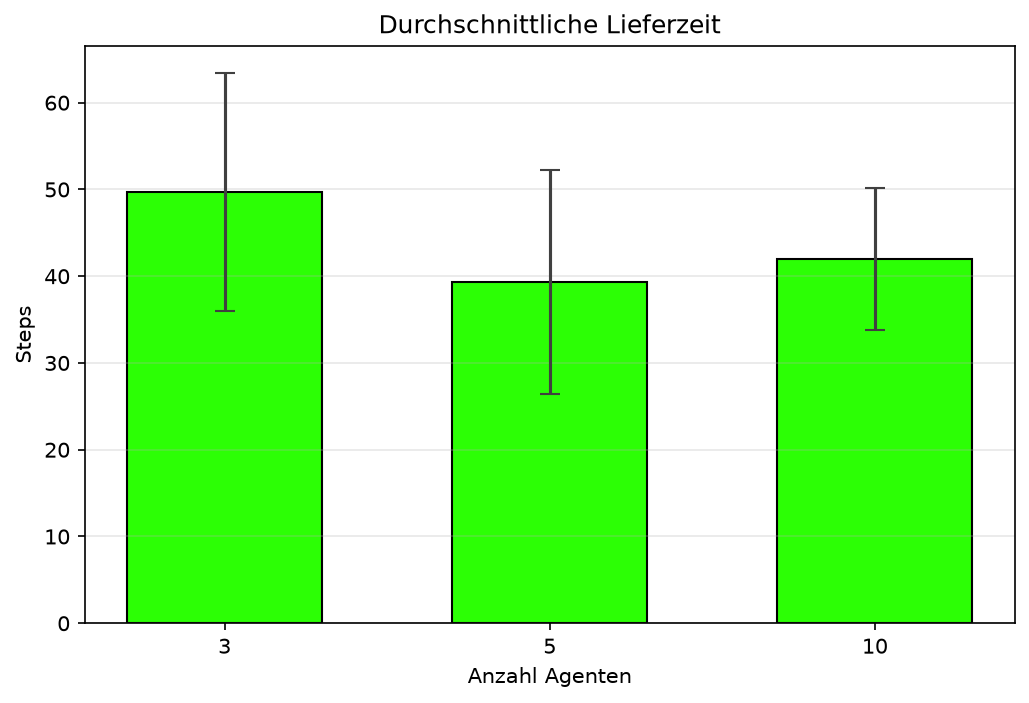
\includegraphics[width=\linewidth]{asset/image/5A-Lieferzeit.png}
        \caption{Durchschnittliche Lieferzeit}
        \label{fig:5a_lieferzeit}
    \end{subfigure}%
    \hfill
    \begin{subfigure}[t]{0.48\textwidth}
        \centering
        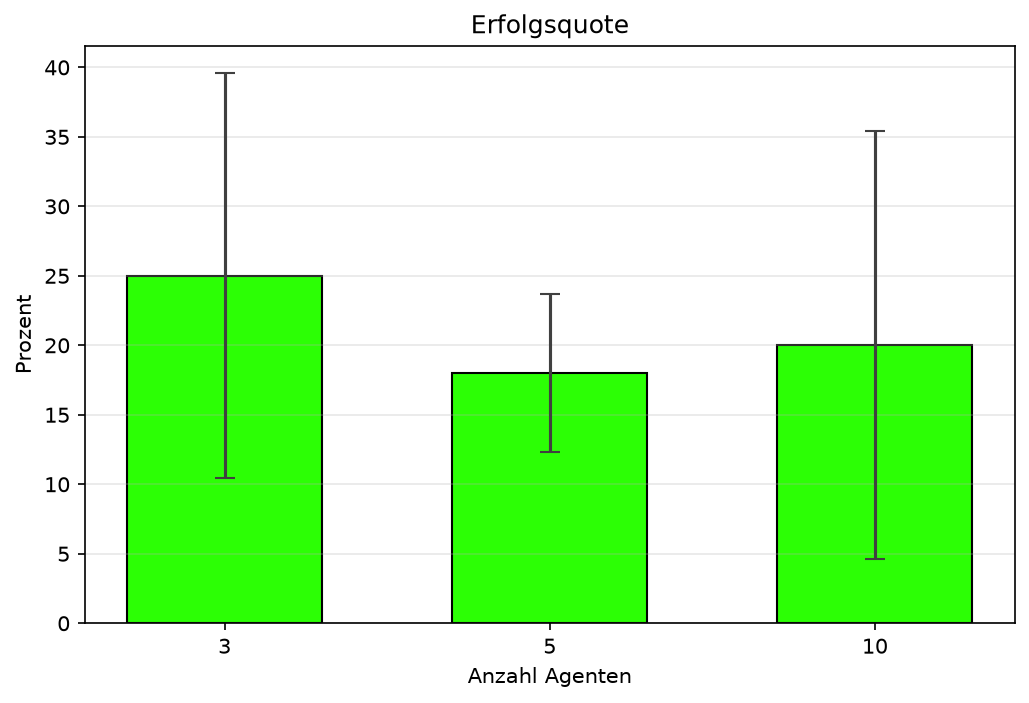
\includegraphics[width=\linewidth]{asset/image/5A-Erfolgsquote.png}
        \caption{Erfolgsquote}
        \label{fig:5a_erfolgsquote}
    \end{subfigure}
    \par\vspace{1em}
    \begin{subfigure}[t]{0.48\textwidth}
        \centering
        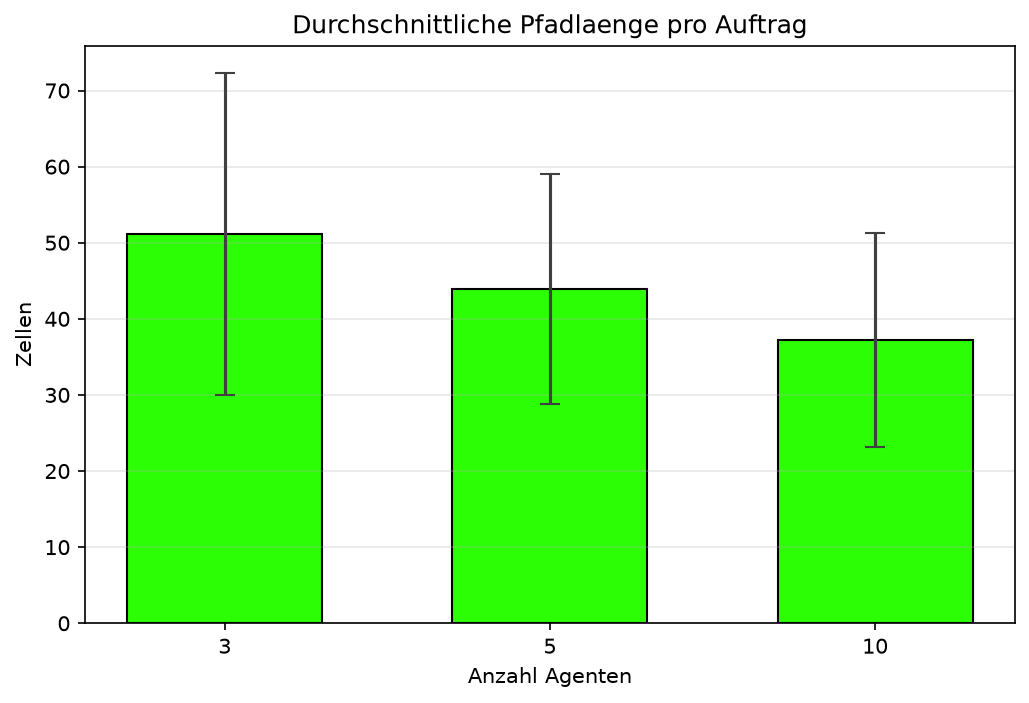
\includegraphics[width=\linewidth]{asset/image/5A-Pfadlaenge.png}
        \caption{Durchschnittliche Pfadlänge}
        \label{fig:5a_pfadlaenge}
    \end{subfigure}
    \caption{Messgrößen pro Agentenkonfiguration}
    \label{fig:5a_metrics}
\end{figure}

\subsubsection{Interpretation der Ergebnisse.}

Die drei Kennzahlen zeigen einen differenzierten Zusammenhang zwischen Agentenanzahl und Systemleistung:

\begin{itemize}
    \item \textbf{Lieferzeit:} Die 5-Agenten-Konfiguration erreicht mit 39{,}4 Steps die niedrigste Lieferzeit. Die 10-Agenten-Konfiguration ist mit 42{,}0 Steps etwas langsamer -- bei vielen Agenten entstehen mehr Konflikte in den 55 Engpässen der Karte (aus Aufgabe~3a), was zu mehr Replanning und damit zu längeren Wegen führt.
    \item \textbf{Erfolgsquote:} Die 3-Agenten-Konfiguration erreicht mit 25\,\% die höchste Erfolgsquote. Dies ist zunächst kontraintuitiv, lässt sich aber durch die geringere Konfliktdichte erklären: Weniger Agenten bedeuten weniger gegenseitige Blockaden, sodass weniger Aufträge an Deadlocks scheitern.
    \item \textbf{Pfadlänge:} Die Pfadlänge sinkt monoton mit steigender Agentenanzahl (51{,}1 \(\to\) 43{,}9 \(\to\) 37{,}2 Zellen). Dies ist ein direkter Effekt der kürzeren Anfahrtswege: Mit mehr Agenten sind die zugewiesenen Agenten im Mittel näher am Depot, sodass die \acs{Astern}-Route kürzer ist.
\end{itemize}

\subsubsection{Fazit.}
Die Ergebnisse zeigen das typische Verhalten eines verteilten Multiagentensystems mit beschränkten Ressourcen: Eine moderate Agentenanzahl (5) liefert die beste Lieferzeit, während bei noch mehr Agenten die Konfliktdichte zunimmt und die Effizienz wieder sinkt. Die niedrige Erfolgsquote (18--25\,\%) ist auf die in Aufgabe~3c bewusst nicht implementierte Ausweich-Logik zurückzuführen -- Agenten, die sich in einem Korridor gegenseitig blockieren, verharren im Deadlock, bis die Deadline abläuft. Diese Konflikte sind das Auswertungsobjekt von Aufgabe~5d.

Die Aggregation über 5 unabhängige Seeds pro Konfiguration liefert belastbare Mittelwerte; die Fehlerbalken zeigen die Streuung zwischen den Läufen -- insbesondere die Erfolgsquote weist eine hohe Varianz auf, was auf die stochastische Natur der Konfliktauflösung zurückzuführen ist.

\paragraph{Anmerkung zum \acs{PROLOG}-Fallback.}
In allen 15 Experimentl\"aufen wurde kein \texttt{subprocess}-Timeout ausgel\"ost; die Fallback-Meldung \texttt{[PROLOG] Fallback auf Python-Logik} erscheint in keiner der dokumentierten Konsolenausgaben. Der Fallback-Pfad aus Aufgabe~4c ist damit implementiert, aber in der Experimentreihe nicht empirisch verifiziert worden. Bei einer produktiven Nutzung mit umfangreicheren Wissensbasen oder langsameren Systemen w\"are eine explizite Protokollierung der Timeouts in den Aggregat-Statistiken empfehlenswert.

% ==============================================================================
% ======================= Aufgabe 5B - A*-Eigenschaften =======================
% ==============================================================================

\section{\acs{Astern}-Eigenschaften \textit{5b}}
\label{sec:aufgabe5b}

\subsection{Aufgabenstellung}

Messen Sie die Eigenschaften der \acs{Astern}-Suche: die Anzahl der expandierten Knoten pro Planung sowie die mittlere und maximale Planungszeit (in ms echter Systemzeit).

\subsection{Theoretische Grundlagen}

Der \acs{Astern}-Algorithmus ist ein \textit{informierter Suchalgorithmus}, dessen Effizienz sich an zwei Größen bemessen lässt: der \textit{Anzahl expandierter Knoten} und der \textit{Laufzeit}. \textcite[S. 21\,f.]{5} beschreibt die Open-Liste als \textit{Prioritätswarteschlange}, aus der in jeder Iteration der Knoten mit dem kleinsten \(f\)-Wert entnommen wird. Jeder so entnommene Knoten wird in die \textit{Closed-Menge} übernommen und seine Nachfolger expandiert. Die Mächtigkeit der Closed-Menge am Ende eines erfolgreichen Laufs entspricht damit exakt der Anzahl der expandierten Knoten und ist ein hardwareunabhängiges Maß für die \textit{Sucheffizienz} eines informierten Verfahrens.

Die \textit{Planungszeit} ist im Gegensatz zur Expansionszahl ein \textit{empirisches} Maß, das von der Hardware, der Python-Interpretation und der aktuellen Systemlast abhängt. Die Aufgabenstellung fordert deshalb ausdrücklich die Messung der \textit{echten Systemzeit} -- also der \textit{Wall-Clock Time} und nicht der reinen CPU-Zeit. In Python ist \texttt{time.perf\_counter()} die geeignete Funktion: Sie liefert eine monotone Uhr mit Sub-Mikrosekunden-Auflösung und ist damit für Mikromessungen präzise genug.

A* hat in der Theorie eine \textit{optimale Effizienz}: Bei zulässiger Heuristik expandiert er keinen Knoten mehr als unbedingt nötig. Die in Aufgabe~3b implementierte \textit{Manhattan-Heuristik} erfüllt diese Zulässigkeit. Dennoch ist die Expansionszahl nicht minimal, weil bei gleichem \(f\)-Wert viele Knoten gleichwertig sind und A* sie alle expandieren muss. Genau diese Beobachtung wird in der Auswertung quantifiziert.

\subsection{Implementierung}

Aufgabe~5b erweitert das bestehende Experiment-Framework aus 5a um eine \acs{Astern}-spezifische Metriken-Erfassung. Die drei Module \texttt{simulation.py}, \texttt{agent.py} und \texttt{experiment.py} werden um Tracking, Aggregation und Visualisierung erweitert. Der \acs{Astern}-Algorithmus selbst bleibt \textbf{unverändert} -- der Rückgabewert \texttt{steps} enthält bereits alle nötigen Informationen.

\paragraph{Design-Entscheidung: Zentrale Metriken-Liste in \texttt{Simulation}.}
Die \acs{Astern}-Messwerte werden nicht pro \texttt{Agent}, sondern zentral in \texttt{Simulation.astar\_metrics} gesammelt. Drei Gründe sprechen dafür: Erstens wird der Agent nicht mit Daten belastet, die nicht zu seinem fachlichen Zustand gehören. Zweitens ist die Aggregation über alle Agenten später ein einzelner Listen-Durchlauf. Drittens ist die Liste konsistent mit dem bereits in 1c etablierten \texttt{\_event\_log}, das ebenfalls simulationsweit geführt wird.

\paragraph{Design-Entscheidung: Messung der Planungszeit im Agenten.}
Die Zeitmessung erfolgt \textit{um den} \texttt{a\_star()}-Aufruf \textit{herum}, nicht innerhalb des Algorithmus. Der Grund: A* ist ein reiner Rechenalgorithmus und sollte frei von Instrumentierung bleiben -- so kann er unverändert in anderen Kontexten (z.\,B.\ später in Tests) genutzt werden. Der Agent als Aufrufer weiß am besten, welche Zeit als \textit{Planungszeit} zu gelten hat: nur der \acs{Astern}-Aufruf, nicht die Log-Ausgabe davor oder danach.

\paragraph{Design-Entscheidung: \texttt{perf\_counter()} statt \texttt{process\_time()}.}
\texttt{time.process\_time()} würde nur die CPU-Zeit messen und I/O-Wartezeiten ignorieren. Da die \acs{Astern}-Suche aber reine CPU-Arbeit ist und die Aufgabenstellung explizit \textit{echte Systemzeit} fordert, ist \texttt{perf\_counter()} die richtige Wahl. Der Overhead von \texttt{perf\_counter()} liegt im Sub-Mikrosekunden-Bereich und ist damit gegenüber den gemessenen Werten von 0{,}1--8\,ms vernachlässigbar.

% ======= config.py – Block 5B =======

\subsubsection{Konfiguration \texttt{config.py} – \acs{Astern}-Metriken-Parameter}

Der neue Konfigurationsblock definiert alle Parameter der \acs{Astern}-Metriken-Erfassung:

\lstinputlisting[
    language=python,
    style=python,
    caption={\acs{Astern}-Metriken-Konfiguration (\texttt{config.py})},
    label={lst:config_5b},
    firstline=498,
    lastline=556
]{asset/code/5B-config.py}

Die Konfiguration umfasst sieben Kategorien:

\begin{itemize}
    \item \textbf{Histogramme} -- Bin-Anzahl (30) und Farben für Histogramm und Boxplot.
    \item \textbf{Ergebnis-Pfade} -- eine CSV und fünf PNG-Pfade (Histogramm/Boxplot für Expansionszahl, Histogramm/Boxplot für Planungszeit, Balken für Maximalzeit).
    \item \textbf{Statistics-Keys} -- Schlüssel für das aggregierte 5b-Metriken-Dictionary.
    \item \textbf{Metric-Keys (intern)} -- Schlüssel der Rohdaten-Struktur (\texttt{expanded}, \texttt{time\_ms}, \texttt{goal}, \texttt{task\_id}, \texttt{step}) sowie der Container-Key \texttt{\_raw\_astar}. Diese Auslagerung folgt dem Single-Source-of-Truth-Prinzip: Wenn die Struktur eines Metrik-Datensatzes geändert wird, muss nur eine Konstante angepasst werden -- nicht vier verstreute Stellen in \texttt{simulation.py} und \texttt{experiment.py}.
    \item \textbf{Zeiteinheiten} -- \texttt{TomaKing5B\_MsPerSecond} (1000.0) als Umrechnungsfaktor zwischen Sekunden und Millisekunden. Die magische Zahl \texttt{1000.0} wäre sonst an zwei Stellen in \texttt{agent.py} dupliziert.
    \item \textbf{CSV} -- Header-Zeile des 5b-Exports (sieben Spalten).
    \item \textbf{Plots} -- Titel, Achsenbeschriftungen, Y-Label.
    \item \textbf{Logging} -- Templates für die aggregierte Ausgabe.
\end{itemize}

Die Validierungsliste in \texttt{validate\_config()} wird um alle neuen Konstanten erweitert (vgl. Abschnitt~\ref{sssec:config_validierung}).

% ======= simulation.py – Imports =======

\subsubsection{Modul \texttt{simulation.py} – Metriken-Tracking und Aggregation}

Die Imports werden um die neuen 5B-Konstanten und das Statistik-Modul der Python-Standardbibliothek erweitert:

\lstinputlisting[
    language=python,
    style=python,
    caption={Statistik-Modul der Python-Standardbibliothek (\texttt{simulation.py})},
    label={lst:sim_imports_5b},
    firstline=10,
    lastline=10
]{asset/code/5B-simulation.py}

\lstinputlisting[
    language=python,
    style=python,
    caption={Erweiterte \texttt{config} Imports (\texttt{simulation.py})},
    label={lst:sim_config_imports_5b},
    firstline=52,
    lastline=66
]{asset/code/5B-simulation.py}

\texttt{statistics} wird für \texttt{mean} und \texttt{median} benötigt. Die Metric-Keys werden aus der Konfiguration importiert, um Hardcoding zu vermeiden.

Der Konstruktor erhält ein neues Feld \texttt{astar\_metrics} als leere Liste:

\lstinputlisting[
    language=python,
    style=python,
    caption={Neues Metriken-Feld im Konstruktor (\texttt{simulation.py})},
    label={lst:sim_ctor_5b},
    firstline=86,
    lastline=86
]{asset/code/5B-simulation.py}

% ======= simulation.py – record_planning =======

Drei neue Methoden implementieren die Erfassung und Aggregation. Die Methode \textbf{\texttt{record\_planning}} nimmt einen einzelnen \acs{Astern}-Aufruf entgegen und schreibt ihn in die Liste:

\lstinputlisting[
    language=python,
    style=python,
    caption={\texttt{record\_planning} (\texttt{simulation.py})},
    label={lst:sim_record_5b},
    firstline=282,
    lastline=295
]{asset/code/5B-simulation.py}

Der Datensatz enthält neben Expansionszahl und Laufzeit auch das Ziel, die Task-ID und den aktuellen Simulationsschritt. Diese Felder werden für die Auswertung nicht direkt benötigt, sind aber für Debugging und eine spätere Konfliktsanalyse (Aufgabe~5d) wertvoll.

Die Methode \textbf{\texttt{get\_astar\_statistics}} aggregiert die Rohdaten zu einem Dictionary:

\lstinputlisting[
    language=python,
    style=python,
    caption={\texttt{get\_astar\_statistics} (\texttt{simulation.py})},
    label={lst:sim_stats_5b},
    firstline=296,
    lastline=320
]{asset/code/5B-simulation.py}

Die Methode liefert einen leeren Default zurück, wenn keine Planungen stattgefunden haben -- dies verhindert einen \texttt{ValueError} in \texttt{statistics.mean} bei Läufen mit sofortigem Abbruch.

Die dritte Methode \textbf{\texttt{get\_astar\_metrics\_raw}} liefert eine \textit{Kopie} der Rohdaten:

\lstinputlisting[
    language=python,
    style=python,
    caption={\texttt{get\_astar\_metrics\_raw} (\texttt{simulation.py})},
    label={lst:sim_raw_5b},
    firstline=321,
    lastline=323
]{asset/code/5B-simulation.py}

Die Kopie ist bewusst gewählt: Der Aufrufer (Experiment) soll die Rohdaten für Histogramme und Boxplots weiterverarbeiten können, ohne die Original-Liste der Simulation zu verändern.

% ======= agent.py – Zeitmessung =======

\subsubsection{Modul \texttt{agent.py} – Zeitmessung um \texttt{a\_star()}}

Der Import wird um \texttt{time} und den Umrechnungsfaktor erweitert:

\lstinputlisting[
    language=python,
    style=python,
    caption={Erweiterte \texttt{time} Import (\texttt{agent.py})},
    label={lst:agent_imports_5b},
    firstline=10,
    lastline=10
]{asset/code/5B-agent.py}

\lstinputlisting[
    language=python,
    style=python,
    caption={Erweiterte \texttt{config} Imports (\texttt{agent.py})},
    label={lst:agent_config_imports_5b},
    firstline=81,
    lastline=82
]{asset/code/5B-agent.py}

Die Methode \textbf{\texttt{\_plan}} wird um die Zeitmessung, Rückgabe-Auswertung und Aufzeichnung erweitert:

\lstinputlisting[
    language=python,
    style=python,
    caption={Erweiterte \texttt{\_plan} (\texttt{agent.py})},
    label={lst:agent_plan_5b},
    firstline=244,
    lastline=252
]{asset/code/5B-agent.py}

Die Änderungen im Detail:

\begin{enumerate}
    \item \textbf{Variable \texttt{steps}}: Der bisher verworfene Rückgabewert \texttt{\_} wird an \texttt{steps} gebunden. Die Liste hat die Form \texttt{(current, f, g, len(open), len(closed))} und enthält damit für jeden Pop-Vorgang einen Eintrag -- ihre Länge entspricht exakt der Anzahl expandierter Knoten.
    \item \textbf{Zeitmessung mit \texttt{perf\_counter()}}: Die beiden Aufrufe liegen unmittelbar vor und nach \texttt{a\_star()}; dazwischen findet keine andere Arbeit statt, sodass die Differenz die reine Planungszeit ist.
    \item \textbf{Multiplikation mit \texttt{TomaKing5B\_MsPerSecond}}: Die Differenz wird in Millisekunden umgerechnet, wobei der Faktor aus der Konfiguration kommt (kein Hardcoding).
\end{enumerate}

Die Methode \textbf{\texttt{\_replan}} wird analog erweitert:

\lstinputlisting[
    language=python,
    style=python,
    caption={Erweiterte \texttt{\_replan} (\texttt{agent.py})},
    label={lst:agent_replan_5b},
    firstline=270,
    lastline=278
]{asset/code/5B-agent.py}

Damit werden alle drei Aufrufstellen des \acs{Astern}-Algorithmus erfasst: die Planung zum Depot, die Planung zum Ziel und das Replanning nach Kollisionen. Der Vollständigkeit halber sei erwähnt, dass in \texttt{decide\_action} und \texttt{\_is\_next\_cell\_blocked} kein \acs{Astern}-Aufruf stattfindet -- sie sind reine Prüfmethoden.

% ======= experiment.py – Auswertung =======

\subsubsection{Modul \texttt{experiment.py} – \acs{Astern}-Auswertung}

Die Imports werden um die 5B-Konstanten erweitert:

\lstinputlisting[
    language=python,
    style=python,
    caption={Erweiterte Imports (\texttt{experiment.py})},
    label={lst:experiment_imports_5b},
    firstline=84,
    lastline=126
]{asset/code/5B-experiment.py}

Die Funktion \textbf{\texttt{\_run\_single}} wird um drei Zeilen erweitert:

\lstinputlisting[
    language=python,
    style=python,
    caption={Erweiterte \texttt{\_run\_single} (\texttt{experiment.py})},
    label={lst:experiment_single_5b},
    firstline=148,
    lastline=151
]{asset/code/5B-experiment.py}

Die drei Statistik-Dictionaries werden per Dict-Merge zusammengeführt. Der Container-Key \texttt{TomaKing5B\_RawAstarKey} (Default: \texttt{"\_raw\_astar"}) transportiert die rohen Messwerte an die Auswertungsfunktionen. Die 5a-CSV ignoriert diesen Schlüssel automatisch, weil sie ihre Felder aus \texttt{TomaKing5A\_CsvHeaderLabels} bezieht.

Fünf neue Funktionen implementieren die Auswertung:

\paragraph{\texttt{\_write\_csv\_5b}.}
Schreibt die aggregierten \acs{Astern}-Kennzahlen als CSV:

\lstinputlisting[
    language=python,
    style=python,
    caption={\texttt{\_write\_csv\_5b} (\texttt{experiment.py})},
    label={lst:experiment_csv_5b},
    firstline=238,
    lastline=251
]{asset/code/5B-experiment.py}

\paragraph{\texttt{\_aggregate\_5b}.}
Aggregiert die \acs{Astern}-Kennzahlen pro Agentenkonfiguration:

\lstinputlisting[
    language=python,
    style=python,
    caption={\texttt{\_aggregate\_5b} (\texttt{experiment.py})},
    label={lst:experiment_aggregate_5b},
    firstline=252,
    lastline=269
]{asset/code/5B-experiment.py}

Für die Maximalkennzahlen wird \texttt{max} über die Runs gebildet -- nicht \texttt{mean}. Die maximale Planungszeit einer Konfiguration ist die maximale über alle 5 Runs, nicht der Mittelwert der fünf Maxima. Diese Wahl entspricht der Aufgabenstellung („maximale Planungszeit``) und ist konsistent mit der klassischen Worst-Case-Bewertung von Suchalgorithmen.

\paragraph{\texttt{\_collect\_5b\_raw}.}
Sammelt die Rohwerte für Histogramme und Boxplots:

\lstinputlisting[
    language=python,
    style=python,
    caption={\texttt{\_collect\_5b\_raw} (\texttt{experiment.py})},
    label={lst:experiment_collect_5b},
    firstline=270,
    lastline=295
]{asset/code/5B-experiment.py}

Die Rohwerte werden in zwei Achsen gesammelt: \texttt{all\_*} für die Gesamtverteilung (Histogramme) und \texttt{per\_config\_*} für den Konfigurationsvergleich (Boxplots). Die Konfigurationsreihenfolge wird aus \texttt{TomaKing5A\_AgentConfigs} übernommen, sodass die X-Achse der Plots konsistent zur 5a-Reihenfolge (3 / 5 / 10 Agenten) ist.

Die drei Plot-Funktionen:

\lstinputlisting[
    language=python,
    style=python,
    caption={Plot-Funktionen (\texttt{experiment.py})},
    label={lst:experiment_plots_5b},
    firstline=296,
    lastline=361
]{asset/code/5B-experiment.py}

\textbf{\texttt{\_make\_histogram\_5b}} erzeugt ein Histogramm mit fester Bin-Anzahl aus der Konfiguration. Die feste Bin-Anzahl (30) ist wichtig für die Vergleichbarkeit mehrerer Läufe -- automatisches Binning (matplotlib-Default) würde je nach Datenmenge unterschiedliche Bins wählen.
\textbf{\texttt{\_make\_boxplot\_5b}} erzeugt einen Boxplot pro Konfiguration. Die Methode verwendet \texttt{tick\_labels} statt des in älteren matplotlib-Versionen üblichen \texttt{labels} -- neuere Versionen haben diesen Parameter umbenannt.
\textbf{\texttt{\_make\_bar\_5b}} erzeugt ein Balkendiagramm der maximalen Planungszeit -- ein einzelner Wert pro Konfiguration.
\textbf{\texttt{\_print\_aggregate\_5b}} gibt die aggregierten \acs{Astern}-Kennzahlen als Tabelle auf der Konsole aus.

Der \texttt{\_\_main\_\_}-Block löst alle 5b-Auswertungsschritte aus:

\lstinputlisting[
    language=python,
    style=python,
    caption={Erweiterter Haupt-Ablauf (\texttt{experiment.py})},
    label={lst:experiment_main_5b},
    firstline=381,
    lastline=394
]{asset/code/5B-experiment.py}

Die 5b-Auswertung läuft unmittelbar nach der 5a-Auswertung. Beide nutzen dieselben 15 Simulationsläufe -- eine zweite Experiment-Serie wäre redundant, da die \acs{Astern}Metriken orthogonal zu den 5a-Kennzahlen sind und aus demselben Simulationslauf extrahiert werden können.

% ======= Refactoring-Übersicht =======

\subsection{Refactoring: Anpassungen an bestehenden Modulen}

Aufgabe~5b erfordert mehrere Anpassungen an bestehenden Modulen:

\begin{table}[H]
    \centering
    \scriptsize
    \begin{tabular}{l l l}
        \toprule
        \textbf{Modul} & \textbf{Änderung} & \textbf{Begründung} \\
        \midrule
        \texttt{config.py} & Block 5B (Histogramme, Pfade, Keys) & Single Source of Truth \\
        \texttt{config.py} & Metric-Keys + \texttt{MsPerSecond} & Hardcoding-Vermeidung \\
        \texttt{simulation.py} & \texttt{astar\_metrics}, \texttt{record\_planning} & Zentrales Metriken-Tracking \\
        \texttt{simulation.py} & \texttt{get\_astar\_statistics}, \texttt{get\_astar\_metrics\_raw} & Aggregation und Rohdaten-Export \\
        \texttt{agent.py} & \texttt{import time} & Für \texttt{perf\_counter()} \\
        \texttt{agent.py} & Timing in \texttt{\_plan}, \texttt{\_replan} & Zeitmessung um A* \\
        \texttt{experiment.py} & \texttt{\_run\_single} um 5b-Stats erweitert & 5a/5b-Daten aus einem Lauf \\
        \texttt{experiment.py} & 5 neue Auswertungsfunktionen & CSV, Aggregation, Plots \\
        \bottomrule
    \end{tabular}
    \caption{Refactoring-Übersicht 5b}
    \label{tab:refactoring_5b}
\end{table}

Der \acs{Astern}Algorithmus (\texttt{astar.py}) bleibt \textbf{unverändert} -- die vorhandene \texttt{steps}-Liste liefert bereits alle benötigten Informationen.

% ======= Ergebnisnachweis =======

\subsection{Ergebnisnachweis}
\label{sssec:astar_5b_nachweis}

Der Nachweis besteht aus drei Teilen: der Einzel-Ergebnis-Tabelle aller 15 Läufe, der aggregierten \acs{Astern}Metriken-Tabelle und den fünf geforderten Plots.

\subsubsection{Teil 1: Einzel-Ergebnisse aller 15 Läufe.}
Die vollständigen \acs{Astern}Metriken der 15 Simulationsläufe sind in Tabelle~\ref{tab:raw_5b} zusammengefasst.

\begin{table}[H]
    \centering
    \small
    \begin{tabular}{r r r r r r r r r}
        \toprule
        \textbf{S} & \textbf{E} & \textbf{Run} & \textbf{Seed} & \textbf{Calls} & \textbf{Exp.Avg} & \textbf{Exp.Max} & \textbf{Zeit Avg [ms]} & \textbf{Zeit Max [ms]} \\
        \midrule
        1 & 2 & 1 & 42 & 284 & 12{,}5 & 44  & 0{,}103 & 2{,}174 \\
        1 & 2 & 2 & 43 & 192 & 16{,}1 & 232 & 0{,}126 & 1{,}956 \\
        1 & 2 & 3 & 44 & 270 & 18{,}4 & 97  & 0{,}178 & 2{,}019 \\
        1 & 2 & 4 & 45 & 194 & 35{,}7 & 103 & 0{,}260 & 2{,}156 \\
        1 & 2 & 5 & 46 & 89  & 60{,}7 & 172 & 0{,}509 & 2{,}414 \\
        \midrule
        2 & 3 & 1 & 42 & 183 & 23{,}6 & 44  & 0{,}171 & 3{,}136 \\
        2 & 3 & 2 & 43 & 250 & 24{,}1 & 215 & 0{,}188 & 2{,}045 \\
        2 & 3 & 3 & 44 & 323 & 28{,}2 & 58  & 0{,}203 & 1{,}943 \\
        2 & 3 & 4 & 45 & 176 & 8{,}5  & 103 & 0{,}094 & 2{,}779 \\
        2 & 3 & 5 & 46 & 62  & 67{,}8 & 172 & 0{,}543 & 3{,}934 \\
        \midrule
        5 & 5 & 1 & 42 & 212 & 21{,}2 & 44  & 0{,}152 & 2{,}658 \\
        5 & 5 & 2 & 43 & 218 & 18{,}5 & 98  & 0{,}153 & 2{,}478 \\
        5 & 5 & 3 & 44 & 223 & 27{,}7 & 97  & 0{,}213 & 2{,}707 \\
        5 & 5 & 4 & 45 & 530 & 8{,}1  & 103 & 0{,}060 & 2{,}114 \\
        5 & 5 & 5 & 46 & 568 & 24{,}8 & 170 & 0{,}182 & 2{,}590 \\
        \bottomrule
    \end{tabular}
    \caption{Einzel-Ergebnisse der 15 Simulationsläufe (S~=~Standard, E~=~Express, Calls~=~\acs{Astern}Aufrufe, Exp.Avg~=~Ø expandierte Knoten, Exp.Max~=~max.\ expandierte Knoten, Zeit Avg/Max~=~mittlere/maximale Planungszeit)}
    \label{tab:raw_5b}
\end{table}

Die volle CSV-Datei liegt als Artefakt bei (\texttt{asset/results/5B-Results.csv}).

\subsubsection{Teil 2: Konsolen-Ausgabe.}
Der 5b-Teil der Experiment-Ausgabe zeigt die aggregierten \acs{Astern}Metriken:

\lstinputlisting[
    style=console,
    caption={Terminal-Ausgabe: 5B-Auswertung},
    label={lst:test_5b_output},
    firstline=1,
    lastline=14
]{asset/code/5B-terminal.tex}

Die aggregierten Ergebnisse sind in Tabelle~\ref{tab:astar_5b} zusammengefasst.

\begin{table}[H]
    \centering
    \begin{tabular}{c r r r r r}
        \toprule
        \textbf{Agenten} & \textbf{Calls} & \textbf{Exp.Avg} & \textbf{Exp.Max} & \textbf{Zeit Avg [ms]} & \textbf{Zeit Max [ms]} \\
        \midrule
        3 (1S/2E)   & 205{,}8 & 28{,}7 & 232 & 0{,}235 & 2{,}414 \\
        5 (2S/3E)   & 198{,}8 & 30{,}4 & 215 & 0{,}240 & 3{,}934 \\
        10 (5S/5E)  & 350{,}2 & 20{,}1 & 170 & 0{,}152 & 2{,}707 \\
        \bottomrule
    \end{tabular}
    \caption{\acs{Astern}Kennzahlen pro Agentenkonfiguration (Mittel bzw.\ Maximum über 5 Runs)}
    \label{tab:astar_5b}
\end{table}

\subsubsection{Teil 3: Plots der \acs{Astern}Eigenschaften.}
Die \acs{Astern}Eigenschaften werden durch fünf Plots dargestellt: zwei Histogramme (Verteilungen), zwei Boxplots (Konfigurationsvergleich) und ein Balkendiagramm (Maximalzeit):

\begin{figure}[H]
    \centering
    \begin{subfigure}[t]{0.48\textwidth}
        \centering
        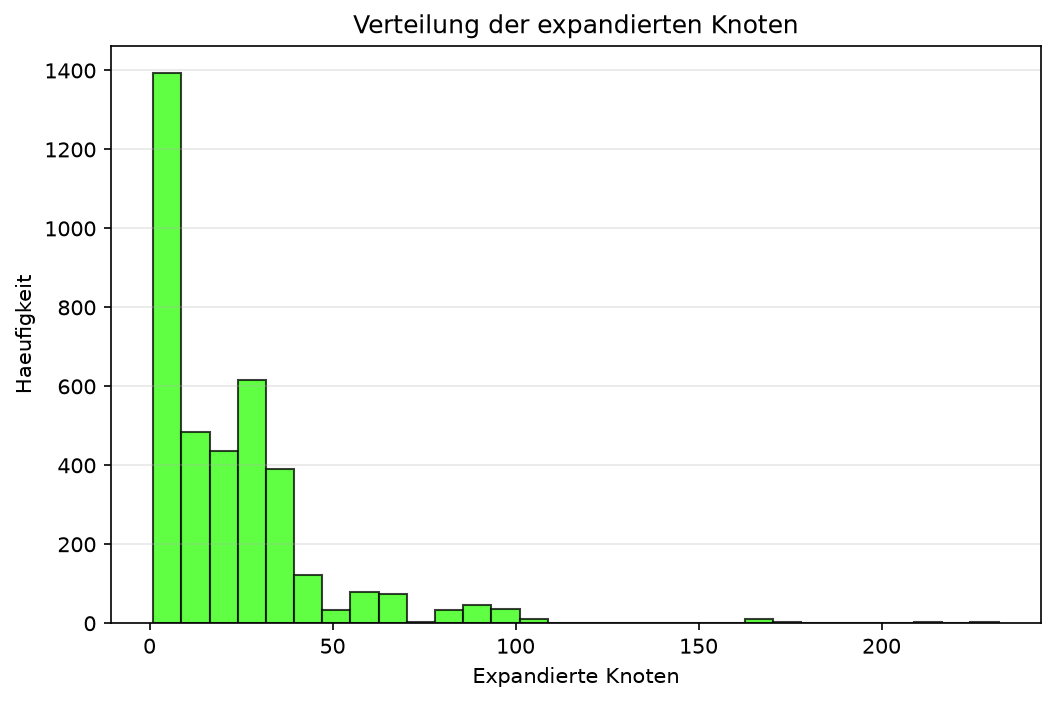
\includegraphics[width=\linewidth]{asset/image/5B-ExpandedHistogram.png}
        \caption{Verteilung der expandierten Knoten}
        \label{fig:5b_expanded_histo}
    \end{subfigure}%
    \hfill
    \begin{subfigure}[t]{0.48\textwidth}
        \centering
        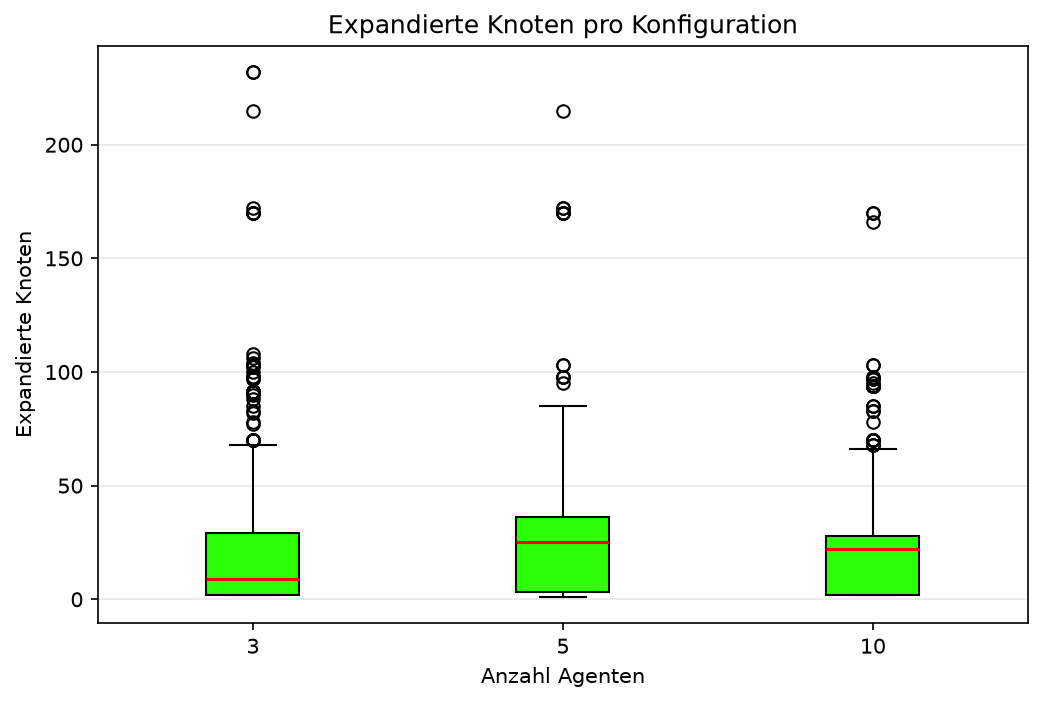
\includegraphics[width=\linewidth]{asset/image/5B-ExpandedBoxplot.png}
        \caption{Expandierte Knoten pro Konfiguration}
        \label{fig:5b_expanded_box}
    \end{subfigure}
    \caption{Expansionszahl des \acs{Astern}Algorithmus}
    \label{fig:5b_expanded}
\end{figure}

\begin{figure}[H]
    \centering
    \begin{subfigure}[t]{0.48\textwidth}
        \centering
        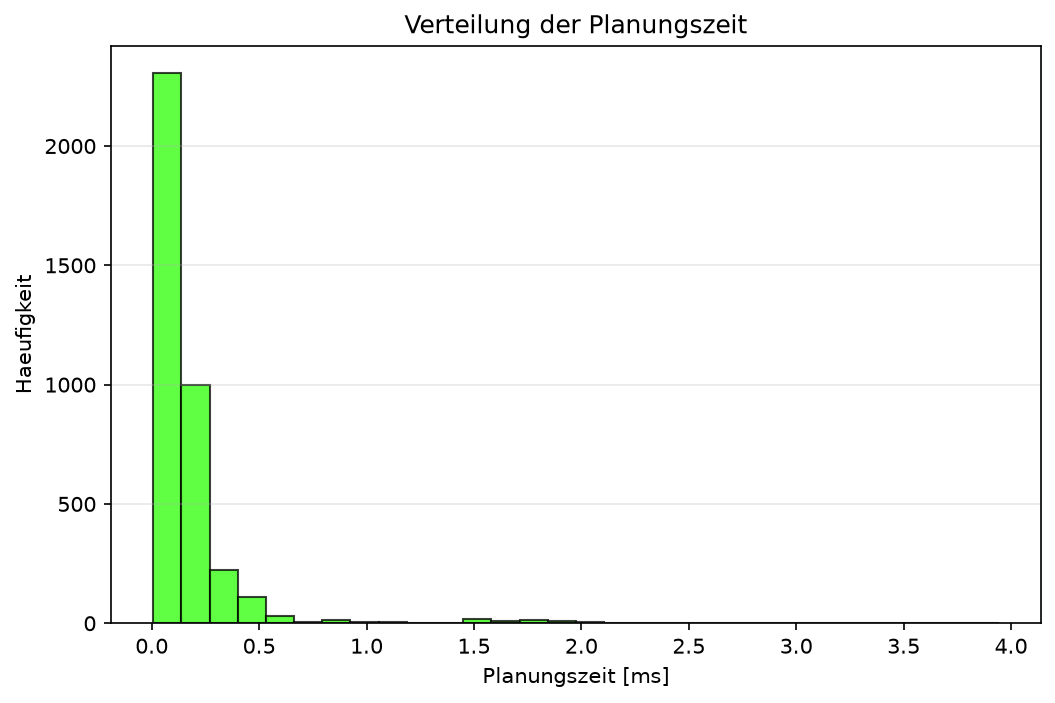
\includegraphics[width=\linewidth]{asset/image/5B-TimeHistogram.png}
        \caption{Verteilung der Planungszeit}
        \label{fig:5b_time_histo}
    \end{subfigure}%
    \hfill
    \begin{subfigure}[t]{0.48\textwidth}
        \centering
        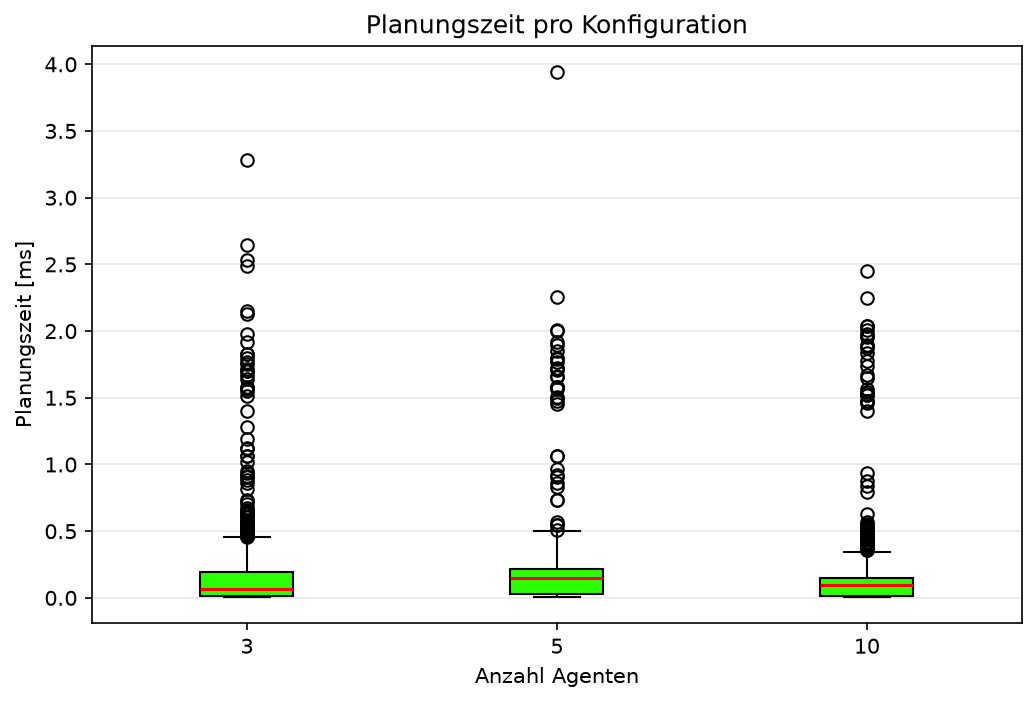
\includegraphics[width=\linewidth]{asset/image/5B-TimeBoxplot.png}
        \caption{Planungszeit pro Konfiguration}
        \label{fig:5b_time_box}
    \end{subfigure}
    \par\vspace{1em}
    \begin{subfigure}[t]{0.48\textwidth}
        \centering
        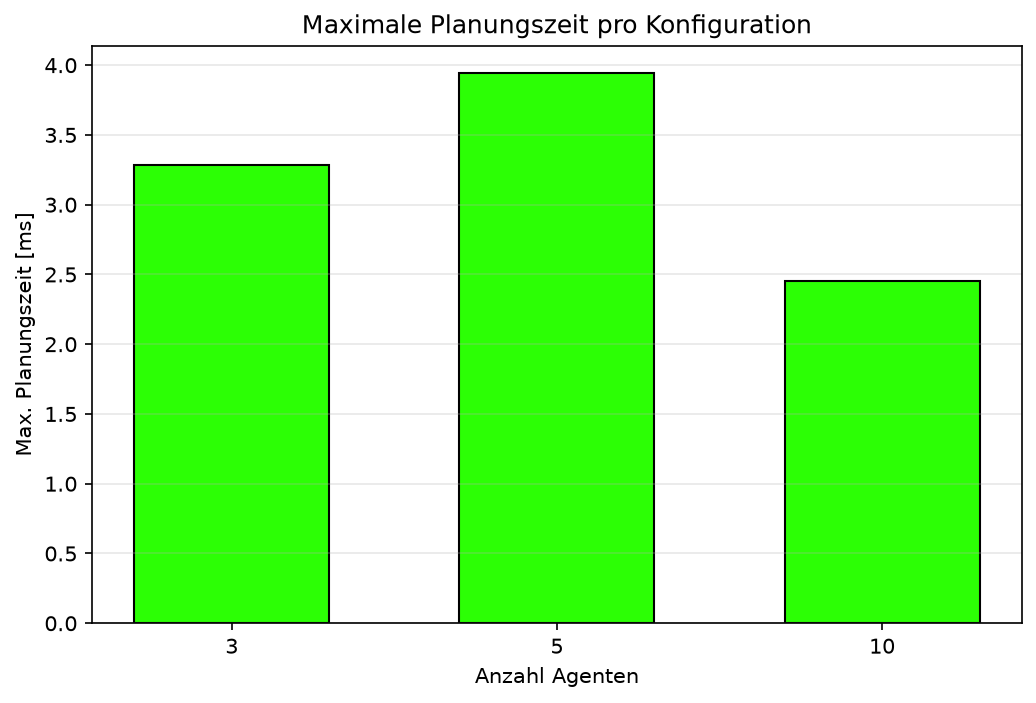
\includegraphics[width=\linewidth]{asset/image/5B-TimeMax.png}
        \caption{Maximale Planungszeit pro Konfiguration}
        \label{fig:5b_time_max}
    \end{subfigure}
    \caption{Planungszeit des \acs{Astern}Algorithmus}
    \label{fig:5b_time}
\end{figure}

\subsubsection{Interpretation der Ergebnisse.}

Die fünf Kennzahlen zeigen ein differenziertes Bild der \acs{Astern}Suche in einem Multiagentensystem:

\textbf{Expansionszahl.} Die durchschnittliche Anzahl expandierter Knoten verläuft nicht-monoton (28{,}7 $\to$ 30{,}4 $\to$ 20{,}1). Der nicht-monotone Verlauf zwischen 3 und 5 Agenten und der deutliche Rückgang bei 10 Agenten lassen sich durch die Verteilung der \acs{Astern}Aufrufe erklären: Bei 10 Agenten dominieren Replanning-Aufrufe (\textbf{350{,}2} Calls gegenüber rund 200 bei 3 und 5 Agenten), die typischerweise auf kurzen Restwegen stattfinden. Eine Planung, die nur noch wenige Zellen bis zum Ziel umfasst, expandiert entsprechend weniger Knoten. Bei 3 und 5 Agenten hingegen überwiegen vollständige Task-Planungen (Depot-Phase und Ziel-Phase), die längere Pfade und damit mehr Expansionen erfordern.

Die \textit{maximale} Expansionszahl ist am höchsten bei 3 Agenten (\textbf{232}) -- ein einzelner Ausreißer in Run~2 (Seed 43), ausgelöst durch eine ungewöhnlich lange Anfahrt. Das Histogramm in Abbildung~\ref{fig:5b_expanded_histo} zeigt die typische Verteilung: eine starke Konzentration im Bereich 0--50 Knoten (kurze Replanning-Pfade), ein zweiter kleinerer Gipfel bei 30--40 Knoten (vollständige Task-Planungen) und eine lange Auslaufzone bis 230 Knoten.

\textbf{Planungszeit.} Die mittlere Planungszeit liegt zwischen \textbf{0{,}152\,ms} (10 Agenten) und \textbf{0{,}240\,ms} (5 Agenten). Der Unterschied zwischen den Konfigurationen ist gering und im Bereich der natürlichen Schwankung -- die absolute Zeit wird von der reinen Python-Laufzeit dominiert, nicht von der Algorithmuskomplexität.

Die \textit{maximale} Planungszeit zeigt kein monotones Muster: Sie ist bei \textbf{5 Agenten} am höchsten (3{,}934\,ms), gefolgt von 10 Agenten (2{,}707\,ms) und 3 Agenten (2{,}414\,ms). Der 5-Agenten-Spitzenwert stammt aus Run~5 (Seed 46) und korreliert \textit{nicht} mit der Expansionszahl -- dieser Lauf hat mit 172 expandierten Knoten nicht den Maximalwert, benötigt aber die höchste Planungszeit. Die reale Systemzeit wird hier offenbar von externen Faktoren beeinflusst (Betriebssystem-Scheduling, Garbage Collection, Hintergrundlast). Die maximale Planungszeit ist daher kein stabiles algorithmus-intrinsisches Maß, sondern eine \textit{Worst-Case-Beobachtung} unter realen Bedingungen.

Das Histogramm in Abbildung~\ref{fig:5b_time_histo} zeigt eine stark rechtsschiefe Verteilung: Der Modus liegt bei 0{,}1--0{,}2\,ms, während Ausreißer bis 3{,}9\,ms reichen. Der Boxplot in Abbildung~\ref{fig:5b_time_box} verdeutlicht die unterschiedliche Streuung der drei Konfigurationen -- die 5-Agenten-Konfiguration hat sowohl den größten Median als auch den größten oberen Whisker.

\textbf{Konfigurationsvergleich.} Die 5-Agenten-Konfiguration zeigt die höchsten Mediane in beiden Boxplots. Die 10-Agenten-Konfiguration weist die niedrigsten mittleren Werte auf -- ein Artefakt der Replanning-Dominanz. Die 3-Agenten-Konfiguration liegt in beiden Boxplots zwischen den beiden anderen.

\subsubsection{Fazit.}

Die Ergebnisse zeigen drei wesentliche Eigenschaften der \acs{Astern}Suche im Multiagentenkontext:

\begin{enumerate}
    \item \textbf{Expansionszahl und Planungszeit sind nicht linear korreliert.} Der 5-Agenten-Ausreißer mit 3{,}934\,ms Planungszeit hat nur 172 expandierte Knoten -- deutlich weniger als der 232-Knoten-Ausreißer bei 3 Agenten, der nur 2{,}414\,ms braucht. Externe Faktoren (CPU-Scheduling, Garbage Collection) dominieren die absolute Zeitmessung. Dies rechtfertigt die Aufgabenstellung, die explizit \textit{echte Systemzeit} fordert: Nur so werden diese realen Effekte sichtbar.
    \item \textbf{Die durchschnittliche Expansionszahl korreliert mit der Aufruf-Mischung, nicht mit der Agentenzahl.} Replanning-Aufrufe auf kurzen Restwegen expandieren weniger Knoten als Erstplanungen auf langen Strecken. Die Agentenzahl wirkt nur indirekt über die relative Häufigkeit von Replanning.
    \item \textbf{Die maximale Planungszeit folgt keinem einfachen Muster.} Zwischen den drei Konfigurationen liegt der Spitzenwert bei 5 Agenten (3{,}934\,ms), während die 10-Agenten-Konfiguration mit 2{,}707\,ms unter diesem Wert bleibt -- trotz doppelter Agentenzahl. Die drei Maximalwerte liegen alle in einem engen Bereich (2{,}4--3{,}9\,ms), was die starke Abhängigkeit von einzelnen Ausreißer-Läufen zeigt.
\end{enumerate}

Die absoluten Zahlen liegen im erwarteten Bereich für einen 70$\times$15-Gittergraphen mit Manhattan-Heuristik: Die typischen Pfadlängen von 25--50 Knoten ergeben Expansionszahlen von 30--230 Knoten. Die Diskrepanz zwischen 25 Pfadknoten und 232 expandierten Knoten (Run~2, 3 Agenten) ist typisch für einen ungewichteten Gitterraum mit vielen gleichwertigen Knoten -- A* muss alle Knoten mit demselben \(f\)-Wert expandieren, um die Optimalität zu garantieren.

Die mit der Agentenzahl stark steigende \acs{Astern}Aufrufrate (205{,}8 $\to$ 198{,}8 $\to$ 350{,}2) deutet auf eine wachsende Zahl von Neuplanungen hin. Diese Konflikte werden in Aufgabe~5d quantitativ analysiert.

% ==============================================================================
% ==================== Aufgabe 5C - Kommunikationsmetriken ====================
% ==============================================================================

\section{Kommunikationsmetriken \textit{5c}}
\label{sec:aufgabe5c}

\subsection{Aufgabenstellung}

Loggen Sie die Kommunikationsmetriken: die durchschnittliche Anzahl von Nachrichten pro Auftrag und die durchschnittliche Anzahl von Bietern pro Auktion.

\subsection{Theoretische Grundlagen}

Das in Aufgabe~2a implementierte \textit{Contract Net Protocol} strukturiert den Nachrichtenaustausch in drei Typen: \textit{Task Announcement} (ANNOUNCE), \textit{Bid} (BID) und \textit{Announced Award} (AWARD). \textcite[S. 30\,f.]{5} beschreibt den Ablauf wie folgt: Ein Depot als Manager beginnt mit der Ausschreibung einer Aufgabe; interessierte Agenten antworten mit einem Gebot; der Manager wählt das beste Gebot und erteilt den Zuschlag an genau einen Gewinner. Dieses Muster ist ein \textit{kooperatives} Protokoll -- der Manager verteilt Arbeit, die Kontraktoren bieten ihre Dienste an.

Der Nachrichtenaufwand dieses Protokolls skaliert mit der Anzahl der beteiligten Agenten. \textcite[S. 32]{5} diskutiert genau diese Skalierungsproblematik am MetaMorph-II-Ansatz: 

\begin{quote}
„Das Problem wird im Umfeld einer Fabrik deutlich, wo Bausubstanz oder elektromagnetische Interferenzen von anderen Maschinen die Kapazität des Kommunikationsweges einschränken, während die meisten Kontraktoren nicht die Rechenleistung haben, um an jedes Angebot evaluieren."
\end{quote}

Die Aufgabenstellung verlangt zwei Kennzahlen, die genau diesen Skalierungseffekt messbar machen:

\begin{itemize}
    \item \textbf{Nachrichten pro Auftrag} -- die Gesamtzahl aller Nachrichten, die über den Lebenszyklus eines Auftrags ausgetauscht werden. Dies ist ein \textit{Kostenmaß} für den Kommunikationskanal.
    \item \textbf{Bieter pro Auktion} -- die Anzahl der eingegangenen Gebote für einen Auftrag. Dies ist ein \textit{Effizienzmaß} für das Bieterverfahren.
\end{itemize}

Beide Größen sind in einem System mit \acs{PROLOG}-Vorfilter (Aufgabe~4c) besonders aussagekräftig, weil der Vorfilter die Menge der erreichbaren und kapazitätsmäßig geeigneten Agenten einschränken kann. Wenn der Vorfilter keine Agenten ausschließt, entspricht die Anzahl der Bieter direkt der Gesamtzahl der Agenten -- eine Beobachtung, die in der Auswertung quantifiziert wird.

\subsection{Implementierung}

Aufgabe~5c erweitert die bestehende Metriken-Erfassung aus 5a und 5b um eine Nachrichten-Ebene. Der zentrale Ansatzpunkt ist die Methode \texttt{Simulation.send\_message}, durch die \textit{alle} Nachrichten zwischen Depots und Agenten fließen. Diese Methode wird um ein Tracking erweitert, das jeden Nachrichtenaustausch protokolliert.

\paragraph{Design-Entscheidung: Zentrales Tracking im Nachrichtenbus.}
Die Nachrichten-Metriken werden im \texttt{send\_message()} der Simulation erfasst -- nicht in den Sendern (Agent oder Depot). Drei Gründe sprechen dafür: Erstens ist \texttt{send\_message()} die einzige Stelle, an der alle Nachrichten vorbeikommen; so kann keine Nachricht vergessen werden. Zweitens werden die Metriken nur dann erfasst, wenn die Nachricht tatsächlich versendet wird -- das entspricht der realen Kanalnutzung. Drittens bleibt die \texttt{Message}-Klasse selbst schlank und frei von Tracking-Logik.

\paragraph{Design-Entscheidung: Filterung nach task\_id.}
Nicht jede Nachricht im System gehört zu einem Auftrag -- theoretisch könnte es später Nachrichten ohne Aufgabenbezug geben. Der Tracking-Filter prüft deshalb, ob die Nachricht einen \texttt{TomaKing2A\_KeyTaskId}-Eintrag im Payload hat. Nur dann wird sie erfasst. Diese Bedingung folgt dem \textit{Single-Responsibility-Prinzip}: Die Kommunikationsmetrik betrifft ausschließlich auftragsbezogene Nachrichten.

\paragraph{Design-Entscheidung: Aggregation über task\_id.}
Beide Kennzahlen leiten sich aus derselben Rohdatenbasis ab: einer Liste von Nachrichten-Datensätzen, gruppiert nach \texttt{task\_id}. Die durchschnittliche Nachrichtenzahl pro Auftrag ist die mittlere Länge dieser Gruppen; die durchschnittliche Bieterzahl pro Auktion ist die mittlere Anzahl von BID-Nachrichten pro Gruppe. Diese doppelte Auswertung derselben Datenbasis vermeidet redundantes Tracking.

% ======= config.py – Block 5C =======

\subsubsection{Konfiguration \texttt{config.py} – Kommunikations-Parameter}

Der neue Konfigurationsblock definiert alle Parameter der Kommunikationsmetriken:

\lstinputlisting[
    language=python,
    style=python,
    caption={Kommunikations-Konfiguration (\texttt{config.py})},
    label={lst:config_5c},
    firstline=558,
    lastline=600
]{asset/code/5C-config.py}

Die Konfiguration umfasst fünf Kategorien:

\begin{itemize}
    \item \textbf{Metric-Keys (intern)} -- Schlüssel der Rohdaten-Struktur (\texttt{task\_id}, \texttt{msg\_type}, \texttt{sender\_id}, \texttt{receiver\_id}, \texttt{step}) sowie der Container-Key \texttt{\_raw\_comm}. Diese Auslagerung folgt dem bereits in 5b etablierten Muster.
    \item \textbf{Ergebnis-Pfade} -- eine CSV und vier PNG-Pfade (je ein Histogramm und Balkendiagramm für beide Kennzahlen).
    \item \textbf{Statistics-Keys} -- Schlüssel für das aggregierte 5c-Metriken-Dictionary.
    \item \textbf{CSV} -- Header-Zeile des 5c-Exports (acht Spalten).
    \item \textbf{Plots} -- Titel und Achsenbeschriftungen.
    \item \textbf{Logging} -- Templates für die aggregierte Ausgabe.
\end{itemize}

Die Validierungsliste in \texttt{validate\_config()} wird um alle neuen Konstanten erweitert (vgl. Abschnitt~\ref{sssec:config_validierung}).

% ======= simulation.py – Imports =======

\subsubsection{Modul \texttt{simulation.py} – Tracking und Aggregation}

Die Imports werden um die neuen 5C-Konstanten sowie um zwei bereits vorhandene 2A-Konstanten erweitert, die nun auch in \texttt{simulation.py} benötigt werden:

\lstinputlisting[
    language=python,
    style=python,
    caption={Erweiterte Imports (\texttt{simulation.py})},
    label={lst:sim_imports_5c},
    firstline=67,
    lastline=82
]{asset/code/5C-simulation.py}

\texttt{TomaKing2A\_MsgBid} wird für den Bieter-Filter in der Aggregation benötigt; \texttt{TomaKing2A\_KeyTaskId} für den Payload-Filter beim Tracking.

Der Konstruktor erhält ein neues Feld \texttt{message\_metrics} als leere Liste:

\lstinputlisting[
    language=python,
    style=python,
    caption={Neues Metriken-Feld im Konstruktor (\texttt{simulation.py})},
    label={lst:sim_ctor_5c},
    firstline=103,
    lastline=103
]{asset/code/5C-simulation.py}

% ======= simulation.py – send_message mit Tracking =======

Die Methode \textbf{\texttt{send\_message}} wird um den Tracking-Block erweitert. Der bestehende Bus-Aufruf bleibt unverändert; darunter wird bei erfüllter Filterbedingung ein neuer Datensatz in \texttt{message\_metrics} angelegt:

\lstinputlisting[
    language=python,
    style=python,
    caption={Erweiterte \texttt{send\_message} mit Tracking (\texttt{simulation.py})},
    label={lst:sim_send_5c},
    firstline=135,
    lastline=142
]{asset/code/5C-simulation.py}

Der Datensatz enthält neben der \texttt{task\_id} auch den Nachrichtentyp, Absender, Empfänger und den Simulationsschritt. Diese Felder werden für die Auswertung nicht alle direkt benötigt -- sie erlauben aber später eine detaillierte Kanalanalyse (z. B. in Aufgabe~5d) und unterstützen Debugging.

% ======= simulation.py – get_communication_statistics =======

Die Methode \textbf{\texttt{get\_communication\_statistics}} aggregiert die Rohdaten nach \texttt{task\_id} und berechnet die beiden geforderten Kennzahlen:

\lstinputlisting[
    language=python,
    style=python,
    caption={\texttt{get\_communication\_statistics} (\texttt{simulation.py})},
    label={lst:sim_stats_5c},
    firstline=350,
    lastline=380
]{asset/code/5C-simulation.py}

Die Aggregation folgt einem zweistufigen Schema: Zuerst werden alle Nachrichten nach \texttt{task\_id} gruppiert (Dictionary mit Listen). Aus diesen Gruppen werden dann zwei Kennzahlen berechnet:

\begin{enumerate}
    \item \textbf{Nachrichten pro Auftrag:} Mittelwert über die Länge jeder Gruppe.
    \item \textbf{Bieter pro Auktion:} Mittelwert über die Anzahl der \texttt{BID}-Nachrichten pro Gruppe. Der Filter nutzt die Konstante \texttt{TomaKing2A\_MsgBid} aus der Konfiguration (kein Hardcoding der Zeichenkette).
\end{enumerate}

Die Default-Rückgabe bei leerer Metriken-Liste verhindert einen \texttt{ValueError} in \texttt{statistics.mean} bei Läufen ohne Auftragsgenerierung.

Die Methode \textbf{\texttt{get\_message\_metrics\_raw}} liefert eine Kopie der Rohdaten:

\lstinputlisting[
    language=python,
    style=python,
    caption={\texttt{get\_message\_metrics\_raw} (\texttt{simulation.py})},
    label={lst:sim_raw_5c},
    firstline=381,
    lastline=383
]{asset/code/5C-simulation.py}

% ======= experiment.py – Imports =======

\subsubsection{Modul \texttt{experiment.py} – Auswertung}

Die Imports werden um die neuen 5C-Konstanten erweitert:

\lstinputlisting[
    language=python,
    style=python,
    caption={Erweiterte Imports (\texttt{experiment.py})},
    label={lst:experiment_imports_5c},
    firstline=127,
    lastline=159
]{asset/code/5C-experiment.py}

\texttt{TomaKing2A\_MsgBid} wird im Rohdaten-Auswerter benötigt und ist bereits über den 2A-Import verfügbar.

% ======= experiment.py – _run_single =======

Die Funktion \textbf{\texttt{\_run\_single}} wird um drei Zeilen erweitert:

\lstinputlisting[
    language=python,
    style=python,
    caption={Erweiterte \texttt{\_run\_single} (\texttt{experiment.py})},
    label={lst:experiment_single_5c},
    firstline=181,
    lastline=188
]{asset/code/5C-experiment.py}

Die 5c-Auswertung nutzt denselben Simulationslauf wie 5a und 5b. Das zurückgegebene Dictionary enthält jetzt vier Statistik-Teile (\texttt{stats\_5a}, \texttt{stats\_5b}, \texttt{stats\_5c}) und zwei Rohdaten-Container (\texttt{\_raw\_astar}, \texttt{\_raw\_comm}). Die Wahl des Variablennamens \texttt{raw\_metrics} (statt \texttt{raw\_astar}) bleibt aus 5b unverändert -- sie ist lokal begrenzt und wird in der Doku zu 5b erklärt.

% ======= experiment.py – neue Funktionen =======

Sechs neue Funktionen implementieren die Auswertung.

\paragraph{\texttt{\_write\_csv\_5c}.}
Schreibt die aggregierten Kommunikationskennzahlen als CSV:

\lstinputlisting[
    language=python,
    style=python,
    caption={\texttt{\_write\_csv\_5c} (\texttt{experiment.py})},
    label={lst:experiment_csv_5c},
    firstline=401,
    lastline=414
]{asset/code/5C-experiment.py}

\paragraph{\texttt{\_aggregate\_5c}.}
Aggregiert die Kommunikationskennzahlen pro Agentenkonfiguration:

\lstinputlisting[
    language=python,
    style=python,
    caption={\texttt{\_aggregate\_5c} (\texttt{experiment.py})},
    label={lst:experiment_aggregate_5c},
    firstline=415,
    lastline=431
]{asset/code/5C-experiment.py}

Anders als bei 5b wird hier für alle vier Kennzahlen der Mittelwert gebildet -- auch für die Total-Werte. Der Grund: Die Gesamtzahl der Nachrichten und Aufträge ist über alle Runs identisch (200 Steps $\times$ 5 Runs, feste Paketintervalle), sodass der Mittelwert dem Einzelwert entspricht.

\paragraph{\texttt{\_collect\_5c\_raw}.}
Sammelt die Rohwerte für Histogramme:

\lstinputlisting[
    language=python,
    style=python,
    caption={\texttt{\_collect\_5c\_raw} (\texttt{experiment.py})},
    label={lst:experiment_collect_5c},
    firstline=432,
    lastline=464
]{asset/code/5C-experiment.py}

Die Funktion gruppiert die rohen Nachrichten aus jedem Run nach \texttt{task\_id} und berechnet zwei Listen: \texttt{msgs\_per\_task} (Länge aller Nachrichten einer Task) und \texttt{bids\_per\_auction} (Anzahl der BID-Nachrichten einer Task). Beide Listen werden sowohl gesamt (\texttt{all\_*}) als auch pro Konfiguration (\texttt{per\_config\_*}) gesammelt.

\paragraph{\texttt{\_make\_histogram\_5b} -- Erweiterung.}
Die 5b-Funktion wird um einen optionalen \texttt{log\_template}-Parameter erweitert, damit sie auch für 5c-Histogramme genutzt werden kann, ohne deren Log-Prefix zu verfälschen:

\lstinputlisting[
    language=python,
    style=python,
    caption={Erweiterte \texttt{\_make\_histogram\_5b} (\texttt{experiment.py})},
    label={lst:experiment_histogram_5c},
    firstline=333,
    lastline=336
]{asset/code/5C-experiment.py}

Der Default-Parameter \texttt{TomaKing5B\_LogPlotSavedTemplate} erhält die Rückwärtskompatibilität für alle 5b-Aufrufe. Die zwei 5c-Histogramm-Aufrufe übergeben explizit \texttt{TomaKing5C\_LogPlotSavedTemplate}, sodass der Terminal-Prefix konsistent zur Aufgabe bleibt.

\paragraph{\texttt{\_make\_bar\_5c}.}
Erzeugt ein Balkendiagramm für eine Kommunikationskennzahl:

\lstinputlisting[
    language=python,
    style=python,
    caption={\texttt{\_make\_bar\_5c} (\texttt{experiment.py})},
    label={lst:experiment_bar_5c},
    firstline=465,
    lastline=480
]{asset/code/5C-experiment.py}

\paragraph{\texttt{\_print\_aggregate\_5c}.}
Gibt die aggregierten Kommunikationsmetriken auf der Konsole aus:

\lstinputlisting[
    language=python,
    style=python,
    caption={\texttt{\_print\_aggregate\_5c} (\texttt{experiment.py})},
    label={lst:experiment_print_5c},
    firstline=481,
    lastline=496
]{asset/code/5C-experiment.py}

% ======= experiment.py – __main__ =======

Der \texttt{\_\_main\_\_}-Block wird um die 5c-Auswertungsschritte erweitert:

\lstinputlisting[
    language=python,
    style=python,
    caption={Erweiterter Haupt-Ablauf (\texttt{experiment.py})},
    label={lst:experiment_main_5c},
    firstline=531,
    lastline=545
]{asset/code/5C-experiment.py}

% ======= Refactoring-Übersicht =======

\subsection{Refactoring: Anpassungen an bestehenden Modulen}

Aufgabe~5c erfordert mehrere Anpassungen an bestehenden Modulen:

\begin{table}[H]
    \centering
    \scriptsize
    \begin{tabular}{l l l}
        \toprule
        \textbf{Modul} & \textbf{Änderung} & \textbf{Begründung} \\
        \midrule
        \texttt{config.py} & Block 5C (Keys, Pfade, Plots) & Single Source of Truth \\
        \texttt{simulation.py} & \texttt{message\_metrics}-Feld & Zentrales Metriken-Tracking \\
        \texttt{simulation.py} & Tracking in \texttt{send\_message} & Erfassung aller Nachrichten \\
        \texttt{simulation.py} & \texttt{get\_communication\_statistics} & Aggregation pro Task \\
        \texttt{simulation.py} & \texttt{get\_message\_metrics\_raw} & Rohdaten-Export \\
        \texttt{experiment.py} & \texttt{\_run\_single} um 5c-Stats erweitert & 5a/5b/5c aus einem Lauf \\
        \texttt{experiment.py} & \texttt{\_make\_histogram\_5b} um \texttt{log\_template} erweitert & Geteilte Nutzung durch 5B und 5C \\
        \texttt{experiment.py} & 6 neue Auswertungsfunktionen & CSV, Aggregation, Plots \\
        \bottomrule
    \end{tabular}
    \caption{Refactoring-Übersicht 5c}
    \label{tab:refactoring_5c}
\end{table}

Der Erweiterung von \texttt{\_make\_histogram\_5b} liegt die Beobachtung zugrunde, dass die Histogramm-Erzeugung eine generische Operation ist: Eingabe-Liste, Datei-Pfad, Titel und Achsenbeschriftung sind die einzigen variablen Aspekte. Der neue \texttt{log\_template}-Parameter macht lediglich den Log-Prefix variabel, ohne die 5b-Aufrufe zu berühren.

% ======= Ergebnisnachweis =======

\subsection{Ergebnisnachweis}
\label{sssec:kommunikation_5c_nachweis}

Der Nachweis besteht aus drei Teilen: der Einzel-Ergebnis-Tabelle aller 15 Läufe, der aggregierten Kommunikationsmetriken-Tabelle und vier Plots.

\subsubsection{Teil 1: Einzel-Ergebnisse aller 15 Läufe.}
Die vollständigen Kommunikationsmetriken der 15 Simulationsläufe sind in Tabelle~\ref{tab:raw_5c} zusammengefasst.

\begin{table}[H]
    \centering
    \small
    \begin{tabular}{r r r r r r r r}
        \toprule
        \textbf{S} & \textbf{E} & \textbf{Run} & \textbf{Seed} & \textbf{Msg/Task} & \textbf{Bieter/Auktion} & \textbf{Msg Total} & \textbf{Tasks} \\
        \midrule
        1 & 2 & 1 & 42 & 7  & 3  & 140 & 20 \\
        1 & 2 & 2 & 43 & 7  & 3  & 140 & 20 \\
        1 & 2 & 3 & 44 & 7  & 3  & 140 & 20 \\
        1 & 2 & 4 & 45 & 7  & 3  & 140 & 20 \\
        1 & 2 & 5 & 46 & 7  & 3  & 140 & 20 \\
        \midrule
        2 & 3 & 1 & 42 & 11 & 5  & 220 & 20 \\
        2 & 3 & 2 & 43 & 11 & 5  & 220 & 20 \\
        2 & 3 & 3 & 44 & 11 & 5  & 220 & 20 \\
        2 & 3 & 4 & 45 & 11 & 5  & 220 & 20 \\
        2 & 3 & 5 & 46 & 11 & 5  & 220 & 20 \\
        \midrule
        5 & 5 & 1 & 42 & 21 & 10 & 420 & 20 \\
        5 & 5 & 2 & 43 & 21 & 10 & 420 & 20 \\
        5 & 5 & 3 & 44 & 21 & 10 & 420 & 20 \\
        5 & 5 & 4 & 45 & 21 & 10 & 420 & 20 \\
        5 & 5 & 5 & 46 & 21 & 10 & 420 & 20 \\
        \bottomrule
    \end{tabular}
    \caption{Einzel-Ergebnisse der 15 Simulationsläufe (S~=~Standard, E~=~Express, Msg/Task~=~Ø Nachrichten pro Auftrag, Bieter/Auktion~=~Ø Bieter pro Auktion, Tasks~=~Anzahl der Aufträge)}
    \label{tab:raw_5c}
\end{table}

Bemerkenswert ist die \textit{Abwesenheit jeglicher Varianz}: Alle fünf Runs einer Konfiguration liefern identische Werte. Dies ist kein Zufallsbefund, sondern ein direkter Effekt des Bieterverfahrens. Das System ist in diesem Szenario \textit{deterministisch}, weil der \acs{PROLOG}-Vorfilter keinen Agenten ausschließt (siehe Interpretation).

Die volle CSV-Datei liegt als Artefakt bei (\texttt{asset/results/5C-Results.csv}).

\subsubsection{Teil 2: Konsolen-Ausgabe.}
Der 5c-Teil der Experiment-Ausgabe zeigt die aggregierten Kommunikationsmetriken:

\lstinputlisting[
    style=console,
    caption={Terminal-Ausgabe: 5C-Auswertung},
    label={lst:test_5c_output},
    firstline=1,
    lastline=13
]{asset/code/5C-terminal.tex}

Die aggregierten Ergebnisse sind in Tabelle~\ref{tab:kommunikation_5c} zusammengefasst.

\begin{table}[H]
    \centering
    \begin{tabular}{c r r r r}
        \toprule
        \textbf{Agenten} & \textbf{Msg/Task} & \textbf{Bieter/Auktion} & \textbf{Msg Total} & \textbf{Tasks} \\
        \midrule
        3 (1S/2E)   & 7  & 3  & 140 & 20 \\
        5 (2S/3E)   & 11 & 5  & 220 & 20 \\
        10 (5S/5E)  & 21 & 10 & 420 & 20 \\
        \bottomrule
    \end{tabular}
    \caption{Kommunikationskennzahlen pro Agentenkonfiguration}
    \label{tab:kommunikation_5c}
\end{table}

Die Einzel- und die Aggregatstabelle sind in diesem Fall \textit{identisch} -- weil die Werte über alle Runs einer Konfiguration deterministisch sind, entspricht der Mittelwert exakt dem Einzelwert.

\subsubsection{Teil 3: Plots der Kommunikationsmetriken.}
Die zwei Kennzahlen werden durch vier Plots dargestellt: je ein Histogramm (Verteilung der Einzelwerte) und je ein Balkendiagramm (aggregierter Durchschnitt pro Konfiguration):

\begin{figure}[H]
    \centering
    \begin{subfigure}[t]{0.48\textwidth}
        \centering
        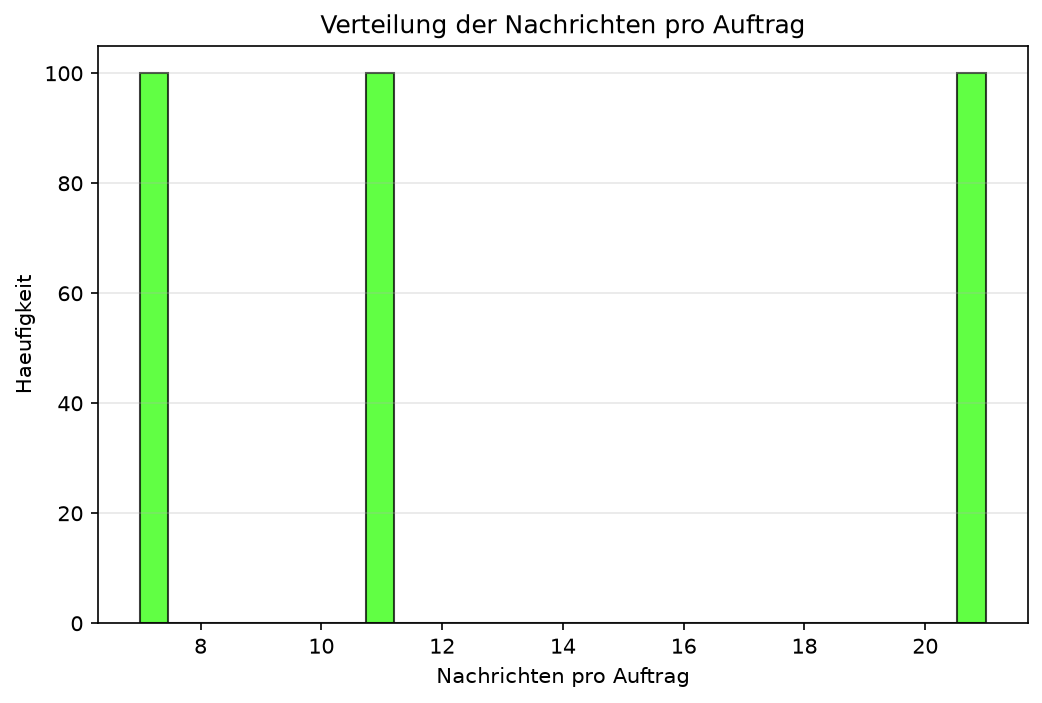
\includegraphics[width=\linewidth]{asset/image/5C-MsgHistogram.png}
        \caption{Verteilung Nachrichten/Auftrag}
        \label{fig:5c_msg_histo}
    \end{subfigure}%
    \hfill
    \begin{subfigure}[t]{0.48\textwidth}
        \centering
        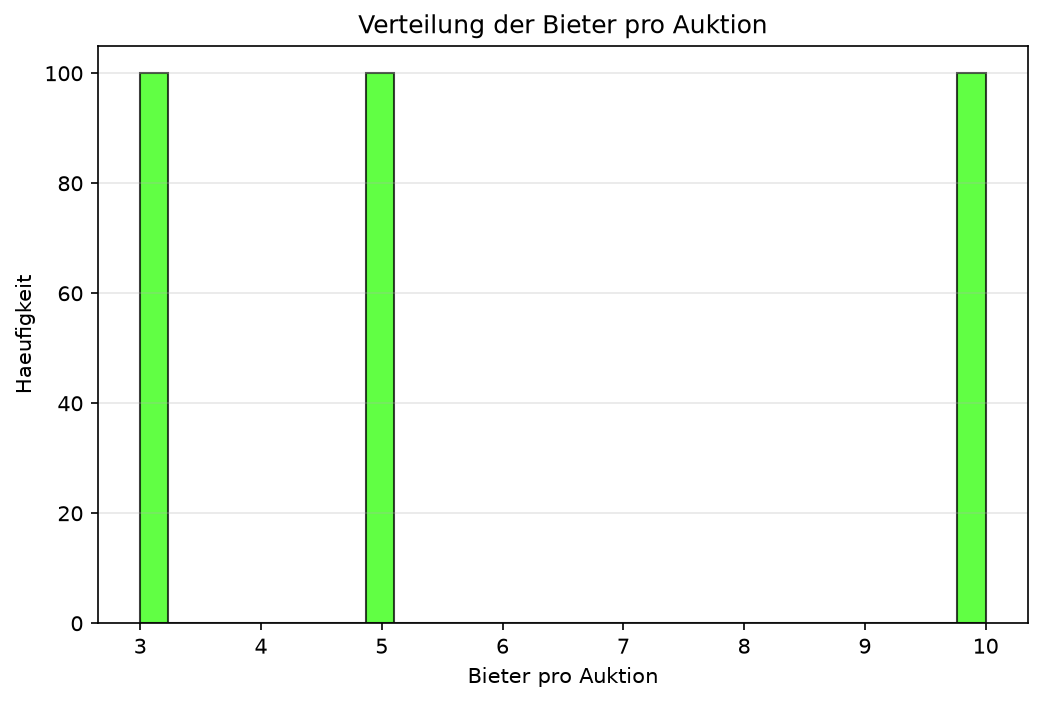
\includegraphics[width=\linewidth]{asset/image/5C-BidHistogram.png}
        \caption{Verteilung Bieter/Auktion}
        \label{fig:5c_bid_histo}
    \end{subfigure}
    \caption{Verteilungen der Kommunikationsmetriken}
    \label{fig:5c_histograms}
\end{figure}

\begin{figure}[H]
    \centering
    \begin{subfigure}[t]{0.48\textwidth}
        \centering
        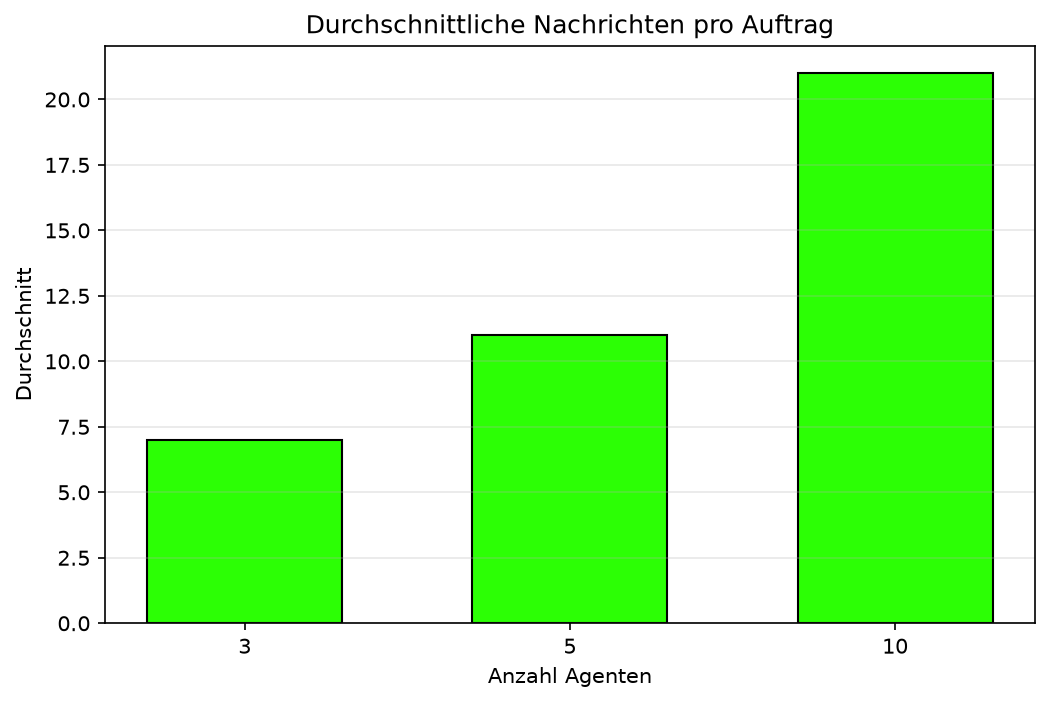
\includegraphics[width=\linewidth]{asset/image/5C-MsgBar.png}
        \caption{Ø Nachrichten/Auftrag}
        \label{fig:5c_msg_bar}
    \end{subfigure}%
    \hfill
    \begin{subfigure}[t]{0.48\textwidth}
        \centering
        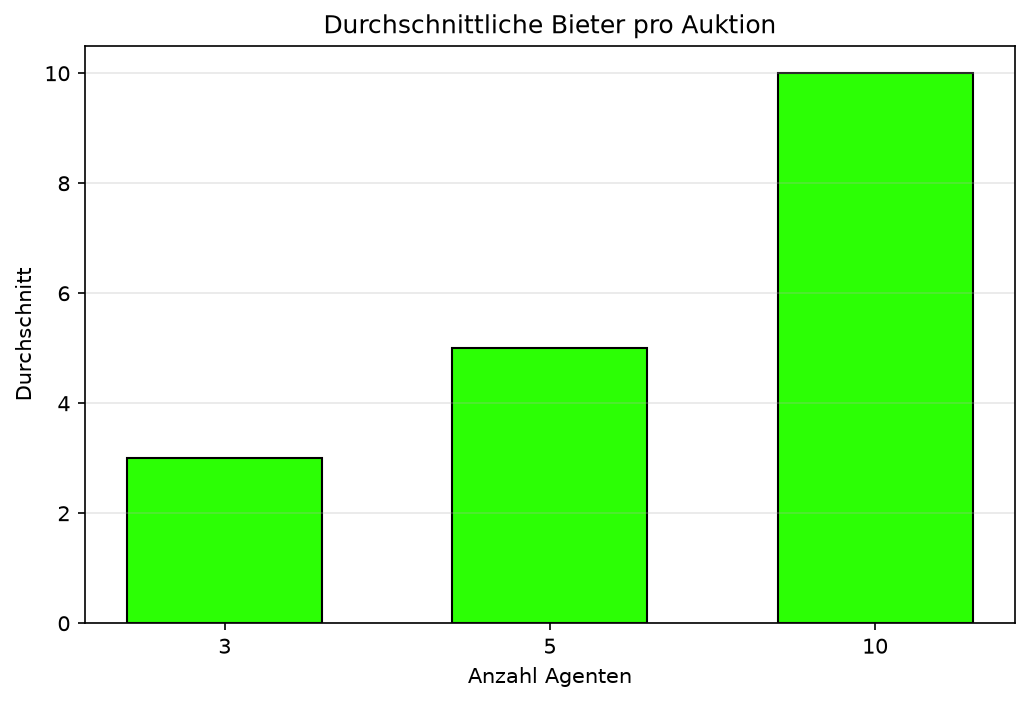
\includegraphics[width=\linewidth]{asset/image/5C-BidBar.png}
        \caption{Ø Bieter/Auktion}
        \label{fig:5c_bid_bar}
    \end{subfigure}
    \caption{Aggregierte Kommunikationskennzahlen pro Konfiguration}
    \label{fig:5c_bars}
\end{figure}

Die beiden Histogramme sind in diesem Fall von eingeschränkter Aussagekraft: Da die Werte pro Konfiguration deterministisch sind, zeigt jedes Histogramm nur drei isolierte Säulen (bei 7/11/21 bzw. 3/5/10) ohne Verteilungscharakter. Die Balkendiagramme hingegen machen den linearen Skalierungseffekt unmittelbar sichtbar.

\subsubsection{Interpretation der Ergebnisse.}

Die beiden Kennzahlen folgen einem \textit{exakt linearen} Skalierungsmuster:

\[
\text{Msg/Task} = 2 \cdot N_{\text{Agenten}} + 1 \qquad
\text{Bieter/Auktion} = N_{\text{Agenten}}
\]

Diese Beziehung lässt sich direkt aus dem \acs{PROLOG}-Vorfilter (Aufgabe~4c) und dem Contract-Net-Protokoll (Aufgabe~2c) herleiten:

\textbf{Nachrichten pro Auftrag.} Für einen Auftrag sendet das Depot zunächst einen ANNOUNCE an jeden eligible Agenten ($N$ Nachrichten). Jeder dieser Agenten antwortet mit einem BID ($N$ Nachrichten). Nach Auswertung sendet das Depot ein AWARD an den Gewinner ($1$ Nachricht). Die Gesamtzahl beträgt damit $2N + 1$. Die Werte 7, 11, 21 für $N = 3, 5, 10$ bestätigen dies exakt.

\textbf{Bieter pro Auktion.} Jeder eligible Agent sendet genau einen BID. Die durchschnittliche Bieterzahl pro Auktion entspricht daher der Anzahl eligible Agenten. Die Werte 3, 5, 10 für $N = 3, 5, 10$ bestätigen dies exakt.

\textbf{Warum keine Varianz?} Der beobachtete Determinismus ist ein direkter Effekt der \texttt{candidate\_agents}-Abfrage: Alle Agenten erfüllen die Kriterien des Vorfilters (\texttt{reachable}, \texttt{Battery > 0}, \texttt{Cargo + 1 =< Capacity}) über den gesamten Simulationsverlauf. Solange der Vorfilter niemanden ausschließt, ist $N_{\text{eligible}} = N_{\text{Agenten}}$ und damit die Kommunikationsmetrik deterministisch. Diese Beobachtung bestätigt auch, dass der in Aufgabe~4c implementierte Vorfilter \textit{korrekt} funktioniert -- er filtert tatsächlich, aber es gibt in diesem Szenario nichts zu filtern.

\textbf{Skalierungsimplikation.} Der Nachrichtenaufwand wächst linear mit der Agentenzahl. Bei 10 Agenten werden pro Auftrag 21 Nachrichten ausgetauscht -- gegenüber 7 bei 3 Agenten eine Verdreifachung. Würde die Zahl der Agenten auf 50 steigen, ergäbe sich ein Aufwand von 101 Nachrichten pro Auftrag. Genau dieser Skalierungseffekt motiviert in der Praxis hierarchische Protokolle wie MetaMorph-II~\cite[S. 32]{5}, bei denen Mediatoren die Broadcast-Phase eingrenzen.

\textbf{Praktische Relevanz.} Im vorliegenden Simulationsszenario mit nur zwei Depots und vier Zielen ist die absolute Nachrichtenzahl (140--420 Nachrichten pro Run über 200 Steps) gering -- der Nachrichtenbus der Simulation ist nicht der Engpass. In einem realen Multiagentensystem mit hunderten Agenten und begrenzter Bandbreite wäre dies jedoch ein dominanter Kostenfaktor.

\subsubsection{Fazit.}

Die Kommunikationsmetriken zeigen das klassische Skalierungsverhalten des Contract-Net-Protokolls: Der Nachrichtenaufwand steigt linear mit der Zahl der beteiligten Agenten, weil sowohl die Ankündigungs- als auch die Gebotsphase als Broadcast erfolgen. Die Ergebnisse sind in diesem Szenario vollständig deterministisch, weil der \acs{PROLOG}-Vorfilter keinen Agenten ausschließt -- ein Hinweis darauf, dass die Vorfilterlogik korrekt arbeitet, aber im vorliegenden Parametersatz (ausreichend Batterie, freie Kapazität, vollständig verbundene Karte) nicht zum Tragen kommt.

Für die Interpretation der Aufgabenstellung ist die zentrale Erkenntnis: Die \textit{Bieterzahl ist der dominante Faktor} für die Nachrichtenlast. Eine Reduktion der eligible-Agenten -- etwa durch strengere Kapazitätsanforderungen oder Batterie-Grenzwerte -- würde die Gesamtzahl der Nachrichten proportional senken. Die Anwendung eines hierarchischen Protokolls (MetaMorph-II mit Mediatoren) wäre die nächste Effizienzstufe, ist aber außerhalb des Aufgabenrahmens.

% ==============================================================================
% =========================== Aufgabe 5D - Konflikte ==========================
% ==============================================================================

\section{Konflikte \textit{5d}}
\label{sec:aufgabe5d}

\subsection{Aufgabenstellung}

Welche Konflikte treten auf? Werten Sie aus, wie viele Kollisionen auftreten (z.~B.\ zwei Agenten wollen in denselben Knoten) und die Anzahl notwendiger Neuplanungen aufgrund von Konflikten.

\subsection{Theoretische Grundlagen}

Konflikte in Multiagentensystemen entstehen, wenn zwei Agenten dieselbe knappe Ressource gleichzeitig beanspruchen. In der Simulation ist die knappste Ressource der \textit{Knoten} -- eine Zelle auf der Karte kann zu jedem Zeitpunkt höchstens von einem Agenten besetzt sein. \textcite[S. 43]{5} beschreibt das Equilibrium als den Gegenpol zum Konflikt:

\begin{quote}
„Equilibria liegen dann vor, wenn sich die Strategien mit den besten Ergebnissen im Gleichgewicht zueinander befinden."
\end{quote}

Ein Konflikt liegt genau dann vor, wenn zwei Agenten dieselbe Zelle anstreben, aber nur eine Strategie realisierbar ist. Das System muss dann eine Lösung finden: Entweder weicht ein Agent aus (\textit{Neuplanung}) oder die Bewegung wird präventiv verhindert (\textit{Kollision}).

\textbf{Strukturelle Kollisionspunkte.} Die in Aufgabe~3a identifizierten \textbf{55 Engpass-Zellen} (Zellen mit maximal zwei Nachbarn) sind die strukturellen Kollisionspunkte der Karte. In einem Engpass ist kein Ausweichmanöver möglich -- die einzige Lösung ist die zeitliche Verschiebung der Bewegung. Diese topologische Einschränkung motiviert die hohen Kollisionszahlen, die in der Auswertung beobachtet werden.

\textbf{Kollision vs.\ Neuplanung.} Beide Begriffe sind konzeptionell verschieden:

\begin{itemize}
    \item \textbf{Kollision:} Ein Agent \textit{will} in eine belegte Zelle ziehen. Dies ist ein \textit{versuchter} Konflikt -- die Bewegung wird präventiv verweigert.
    \item \textbf{Neuplanung:} Ein Agent erkennt, dass seine aktuelle Route blockiert ist, und berechnet eine neue Route. Dies ist die \textit{Reaktion} auf einen Konflikt.
\end{itemize}

\subsection{Implementierung}

Aufgabe~5d erweitert die Simulation um ein zentrales Konflikt-Tracking. Die Erfassung erfolgt in zwei Momenten: beim präventiven Blockade-Check in \texttt{try\_move} (Kollision) und beim Aufruf der Neuplanungsmethode \texttt{\_replan} (Neuplanung). Der \acs{Astern}Algorithmus und die Graph-Struktur bleiben \textbf{unverändert}.

\paragraph{Design-Entscheidung: Zentrales Tracking in \texttt{Simulation}.}
Die Zähler \texttt{collision\_count} und \texttt{replan\_count} werden in der \texttt{Simulation}-Instanz geführt -- konsistent mit \texttt{astar\_metrics} (5b) und \texttt{message\_metrics} (5c). Zusätzlich werden Event-Listen geführt, sodass eine detaillierte Feinanalyse (z.~B.\ welche Engpässe besonders kollisionsanfällig sind) möglich bleibt.

\paragraph{Design-Entscheidung: Zählung nur bei echter Blockade.}
Der \texttt{record\_collision}-Aufruf steht genau an der Stelle, an der \texttt{try\_move} die Bewegung verweigert -- also \textit{nach} der Bestätigung, dass die Zielzelle von einem anderen Agenten belegt ist. Bewegungen auf Wände (\texttt{not walkable}) zählen \textbf{nicht} als Kollision, weil sie kein Agent-Agent-Konflikt sind, sondern ein Planungsfehler.

\paragraph{Design-Entscheidung: Neuplanung vor dem early-return.}
Der \texttt{record\_replan}-Aufruf steht in \texttt{\_replan} \textit{vor} dem early-return, der bei unveränderter Route ausgelöst wird. Damit wird jede \textit{notwendige} Neuplanung gezählt -- auch wenn A* zufällig dieselbe Route zurückliefert. Diese Wahl folgt dem Wortlaut der Aufgabenstellung („Anzahl notwendiger Neuplanungen``), nicht dem Ergebnis der Neuplanung.

% ======= config.py – Block 5D =======

\subsubsection{Konfiguration \texttt{config.py} – Konflikt-Parameter}

Der neue Konfigurationsblock definiert alle Parameter des Konflikt-Trackings:

\lstinputlisting[
    language=python,
    style=python,
    caption={Konflikt-Konfiguration (\texttt{config.py})},
    label={lst:config_5d},
    firstline=602,
    lastline=644
]{asset/code/5D-config.py}

Die Konfiguration umfasst fünf Kategorien:

\begin{itemize}
    \item \textbf{Metric-Keys (intern)} -- Schlüssel der Event-Struktur (\texttt{agent\_id}, \texttt{target}, \texttt{goal}, \texttt{step}) sowie die Container-Keys \texttt{\_raw\_collisions} und \texttt{\_raw\_replans}.
    \item \textbf{Guards} -- \texttt{TomaKing5D\_MinStepCount} (1) verhindert eine Division durch null in der Per-Step-Rate bei Läufen mit Schrittanzahl~0.
    \item \textbf{Ergebnis-Pfade} -- eine CSV und drei PNG-Pfade.
    \item \textbf{Statistics-Keys} -- Schlüssel für absolute und normalisierte Kennzahlen.
    \item \textbf{Plots} -- Titel, Y-Achsen-Beschriftung, Legendeneinträge und Farbe der zweiten Serie im Doppelbalkendiagramm.
    \item \textbf{Logging} -- Templates für CSV-Bestätigung, Aggregations-Header und Tabellenzeilen.
\end{itemize}

Die Validierungsliste in \texttt{validate\_config()} wird um alle neuen Konstanten erweitert.

% ======= simulation.py – Imports =======

\subsubsection{Modul \texttt{simulation.py} – Tracking und Aggregation}

Die Imports werden um die neuen 5D-Konstanten erweitert:

\lstinputlisting[
    language=python,
    style=python,
    caption={Erweiterte Imports (\texttt{simulation.py})},
    label={lst:sim_imports_5d},
    firstline=83,
    lastline=94
]{asset/code/5D-simulation.py}

Der Konstruktor erhält vier neue Felder:

\lstinputlisting[
    language=python,
    style=python,
    caption={Neue Felder im Konstruktor (\texttt{simulation.py})},
    label={lst:sim_ctor_5d},
    firstline=116,
    lastline=119
]{asset/code/5D-simulation.py}

Fünf neue Methoden implementieren Erfassung und Aggregation. Die Methode \textbf{\texttt{record\_collision}} registriert einen Kollisionsversuch:

\lstinputlisting[
    language=python,
    style=python,
    caption={\texttt{record\_collision} (\texttt{simulation.py})},
    label={lst:sim_collision_5d},
    firstline=401,
    lastline=412
]{asset/code/5D-simulation.py}

Die Methode \textbf{\texttt{record\_replan}} registriert eine Neuplanung:

\lstinputlisting[
    language=python,
    style=python,
    caption={\texttt{record\_replan} (\texttt{simulation.py})},
    label={lst:sim_replan_5d},
    firstline=412,
    lastline=420
]{asset/code/5D-simulation.py}

Die Methode \textbf{\texttt{get\_conflict\_statistics}} liefert die aggregierten Kennzahlen:

\lstinputlisting[
    language=python,
    style=python,
    caption={\texttt{get\_conflict\_statistics} (\texttt{simulation.py})},
    label={lst:sim_stats_5d},
    firstline=421,
    lastline=429
]{asset/code/5D-simulation.py}

Die Per-Step-Raten sind normalisierte Kennzahlen: Sie erlauben einen direkten Vergleich zwischen Läufen mit unterschiedlicher Simulationsdauer. Der Guard \texttt{max(self.step\_count, TomaKing5D\_MinStepCount)} schützt gegen eine Division durch null (in der Praxis immer $\geq$~\texttt{StepCount}).

Die beiden Methoden \textbf{\texttt{get\_collision\_events\_raw}} und \textbf{\texttt{get\_replan\_events\_raw}} liefern Kopien der Event-Listen:

\lstinputlisting[
    language=python,
    style=python,
    caption={Rohdaten-Export (\texttt{simulation.py})},
    label={lst:sim_raw_5d},
    firstline=430,
    lastline=434
]{asset/code/5D-simulation.py}

% ======= agent.py – Tracking-Aufrufe =======

\subsubsection{Modul \texttt{agent.py} – Tracking-Aufrufe}

Zwei Aufrufe werden ergänzt.

In \textbf{\texttt{try\_move}} wird beim Blockade-Fall die Kollision registriert:

\lstinputlisting[
    language=python,
    style=python,
    caption={Erweiterte \texttt{try\_move} (\texttt{agent.py})},
    label={lst:agent_trymove_5d},
    firstline=142,
    lastline=142
]{asset/code/5D-agent.py}

In \textbf{\texttt{\_replan}} wird jede Neuplanung registriert, direkt nach der Zielbestimmung:

\lstinputlisting[
    language=python,
    style=python,
    caption={Erweiterte \texttt{\_replan} (\texttt{agent.py})},
    label={lst:agent_replan_5d},
    firstline=271,
    lastline=271
]{asset/code/5D-agent.py}

Der Aufruf steht \textbf{vor} dem early-return für unveränderte Routen -- damit entspricht die gezählte Zahl jeder tatsächlich notwendigen Neuplanung.

% ======= experiment.py – Auswertung =======

\subsubsection{Modul \texttt{experiment.py} – Auswertung}

Die Imports werden um die neuen 5D-Konstanten erweitert:

\lstinputlisting[
    language=python,
    style=python,
    caption={Erweiterte Imports (\texttt{experiment.py})},
    label={lst:experiment_imports_5d},
    firstline=160,
    lastline=188
]{asset/code/5D-experiment.py}

Die Funktion \textbf{\texttt{\_run\_single}} wird um 5D-Daten erweitert:

\lstinputlisting[
    language=python,
    style=python,
    caption={Erweiterte \texttt{\_run\_single} (\texttt{experiment.py})},
    label={lst:experiment_single_5d},
    firstline=213,
    lastline=222
]{asset/code/5D-experiment.py}

Fünf neue Funktionen:

\paragraph{\texttt{\_write\_csv\_5d}.}
Schreibt die aggregierten Konfliktkennzahlen als CSV:

\lstinputlisting[
    language=python,
    style=python,
    caption={\texttt{\_write\_csv\_5d} (\texttt{experiment.py})},
    label={lst:experiment_csv_5d},
    firstline=532,
    lastline=545
]{asset/code/5D-experiment.py}

\paragraph{\texttt{\_aggregate\_5d}.}
Aggregiert die Konfliktkennzahlen pro Agentenkonfiguration:

\lstinputlisting[
    language=python,
    style=python,
    caption={\texttt{\_aggregate\_5d} (\texttt{experiment.py})},
    label={lst:experiment_aggregate_5d},
    firstline=546,
    lastline=562
]{asset/code/5D-experiment.py}

Alle vier Kennzahlen werden gemittelt -- auch die Per-Step-Raten, weil sie pro Run berechnet und anschließend aggregiert werden. Dies ist konsistent mit 5a und 5b.

\paragraph{\texttt{\_make\_bar\_5d}.}
Erzeugt ein einfaches Balkendiagramm für eine Konfliktkennzahl:

\lstinputlisting[
    language=python,
    style=python,
    caption={\texttt{\_make\_bar\_5d} (\texttt{experiment.py})},
    label={lst:experiment_bar_5d},
    firstline=563,
    lastline=578
]{asset/code/5D-experiment.py}

\paragraph{\texttt{\_make\_double\_bar\_5d}.}
Erzeugt einen Doppelbalken-Vergleich für Kollisionen und Neuplanungen:

\lstinputlisting[
    language=python,
    style=python,
    caption={\texttt{\_make\_double\_bar\_5d} (\texttt{experiment.py})},
    label={lst:experiment_doublebar_5d},
    firstline=579,
    lastline=606
]{asset/code/5D-experiment.py}

Die zwei Serien werden um $\pm$\texttt{width/2} versetzt um die gleiche X-Position, sodass sie nebeneinander liegen statt sich zu überlagern. Der Vorteil dieser Darstellung: Bei übereinstimmenden Werten (siehe Auswertung) sind die zwei Balken exakt gleich hoch und machen die 1:1-Beziehung unmittelbar sichtbar.

\paragraph{\texttt{\_print\_aggregate\_5d}.}
Gibt die aggregierten Konfliktkennzahlen auf der Konsole aus:

\lstinputlisting[
    language=python,
    style=python,
    caption={\texttt{\_print\_aggregate\_5d} (\texttt{experiment.py})},
    label={lst:experiment_print_5d},
    firstline=607,
    lastline=622
]{asset/code/5D-experiment.py}

Der \texttt{\_\_main\_\_}-Block wird um die 5D-Aufrufe erweitert:

\lstinputlisting[
    language=python,
    style=python,
    caption={Erweiterter Haupt-Ablauf (\texttt{experiment.py})},
    label={lst:experiment_main_5d},
    firstline=672,
    lastline=683
]{asset/code/5D-experiment.py}

% ======= Refactoring-Übersicht =======

\subsection{Refactoring: Anpassungen an bestehenden Modulen}

\begin{table}[H]
    \centering
    \scriptsize
    \begin{tabular}{l l l}
        \toprule
        \textbf{Modul} & \textbf{Änderung} & \textbf{Begründung} \\
        \midrule
        \texttt{config.py} & Block 5D (Keys, Pfade, Plots) & Single Source of Truth \\
        \texttt{simulation.py} & Vier Felder im Konstruktor & Zähler und Event-Listen \\
        \texttt{simulation.py} & \texttt{record\_collision}, \texttt{record\_replan} & Zentrale Erfassung \\
        \texttt{simulation.py} & \texttt{get\_conflict\_statistics} & Aggregation \\
        \texttt{agent.py} & Tracking in \texttt{try\_move} & Kollisions-Erfassung \\
        \texttt{agent.py} & Tracking in \texttt{\_replan} & Neuplanungs-Erfassung \\
        \texttt{experiment.py} & \texttt{\_run\_single} um 5d-Daten & Konsistenz mit 5a--5c \\
        \texttt{experiment.py} & 5 neue Auswertungsfunktionen & CSV, Aggregation, Plots \\
        \bottomrule
    \end{tabular}
    \caption{Refactoring-Übersicht 5d}
    \label{tab:refactoring_5d}
\end{table}

Der \acs{Astern}Algorithmus (\texttt{astar.py}) und die Graph-Struktur (\texttt{graph.py}) bleiben \textbf{unverändert}.

% ======= Ergebnisnachweis =======

\subsection{Ergebnisnachweis}
\label{sssec:konflikte_5d_nachweis}

Der Nachweis besteht aus drei Teilen: der Einzel-Ergebnis-Tabelle aller 15 Läufe, der aggregierten Konfliktkennzahlen-Tabelle und drei Plots.

\subsubsection{Teil 1: Einzel-Ergebnisse aller 15 Läufe.}
Die vollständigen Konfliktkennzahlen der 15 Simulationsläufe sind in Tabelle~\ref{tab:raw_5d} zusammengefasst.

\begin{table}[H]
    \centering
    \small
    \begin{tabular}{r r r r r r r r}
        \toprule
        \textbf{S} & \textbf{E} & \textbf{Run} & \textbf{Seed} & \textbf{Kollisionen} & \textbf{Neuplanungen} & \textbf{Koll./Step} & \textbf{Repl./Step} \\
        \midrule
        1 & 2 & 1 & 42 & 257 & 257 & 1{,}285 & 1{,}285 \\
        1 & 2 & 2 & 43 & 174 & 174 & 0{,}870 & 0{,}870 \\
        1 & 2 & 3 & 44 & 243 & 243 & 1{,}215 & 1{,}215 \\
        1 & 2 & 4 & 45 & 180 & 180 & 0{,}900 & 0{,}900 \\
        1 & 2 & 5 & 46 & 74  & 74  & 0{,}370 & 0{,}370 \\
        \midrule
        2 & 3 & 1 & 42 & 162 & 162 & 0{,}810 & 0{,}810 \\
        2 & 3 & 2 & 43 & 231 & 231 & 1{,}155 & 1{,}155 \\
        2 & 3 & 3 & 44 & 304 & 304 & 1{,}520 & 1{,}520 \\
        2 & 3 & 4 & 45 & 157 & 157 & 0{,}785 & 0{,}785 \\
        2 & 3 & 5 & 46 & 45  & 45  & 0{,}225 & 0{,}225 \\
        \midrule
        5 & 5 & 1 & 42 & 188 & 188 & 0{,}940 & 0{,}940 \\
        5 & 5 & 2 & 43 & 197 & 197 & 0{,}985 & 0{,}985 \\
        5 & 5 & 3 & 44 & 195 & 195 & 0{,}975 & 0{,}975 \\
        5 & 5 & 4 & 45 & 510 & 510 & 2{,}550 & 2{,}550 \\
        5 & 5 & 5 & 46 & 550 & 550 & 2{,}750 & 2{,}750 \\
        \bottomrule
    \end{tabular}
    \caption{Einzel-Ergebnisse der 15 Simulationsläufe (S~=~Standard, E~=~Express, Koll./Step~=~Kollisionen pro Simulationsschritt, Repl./Step~=~Neuplanungen pro Simulationsschritt)}
    \label{tab:raw_5d}
\end{table}

Die auffälligste Beobachtung: \textbf{Kollisionen und Neuplanungen sind in jedem der 15 Läufe exakt identisch}. Diese 1:1-Beziehung ist kein Zufall, sondern ein direkter Effekt der Code-Architektur (siehe Interpretation).

Die volle CSV-Datei liegt als Artefakt bei (\texttt{asset/results/5D-Results.csv}). In der CSV-Datei sind die Per-Step-Werte im angelsächsischen Format mit Punkt als Dezimaltrenner gespeichert; die Darstellung in Tabelle~\ref{tab:raw_5d} verwendet Komma als Dezimaltrenner, konsistent zu den vorigen Aufgaben.

\subsubsection{Teil 2: Konsolen-Ausgabe.}
Der 5d-Teil der Experiment-Ausgabe zeigt die aggregierten Konfliktkennzahlen:

\lstinputlisting[
    style=console,
    caption={Terminal-Ausgabe: 5D-Auswertung},
    label={lst:test_5d_output},
    firstline=1,
    lastline=12
]{asset/code/5D-terminal.tex}

Die aggregierten Ergebnisse sind in Tabelle~\ref{tab:konflikte_5d} zusammengefasst.

\begin{table}[H]
    \centering
    \begin{tabular}{c r r r r}
        \toprule
        \textbf{Agenten} & \textbf{Kollisionen} & \textbf{Neuplanungen} & \textbf{Koll./Step} & \textbf{Repl./Step} \\
        \midrule
        3 (1S/2E)   & 185{,}6 & 185{,}6 & 0{,}928 & 0{,}928 \\
        5 (2S/3E)   & 179{,}8 & 179{,}8 & 0{,}899 & 0{,}899 \\
        10 (5S/5E)  & 328{,}0 & 328{,}0 & 1{,}640 & 1{,}640 \\
        \bottomrule
    \end{tabular}
    \caption{Konfliktkennzahlen pro Agentenkonfiguration (Mittel über 5 Runs)}
    \label{tab:konflikte_5d}
\end{table}

\subsubsection{Teil 3: Plots der Konfliktkennzahlen.}
Die zwei Kennzahlen werden durch drei Plots dargestellt: zwei einfache Balkendiagramme (Kollisionen, Neuplanungen) und ein Doppelbalken-Vergleich.

\begin{figure}[H]
    \centering
    \begin{subfigure}[t]{0.48\textwidth}
        \centering
        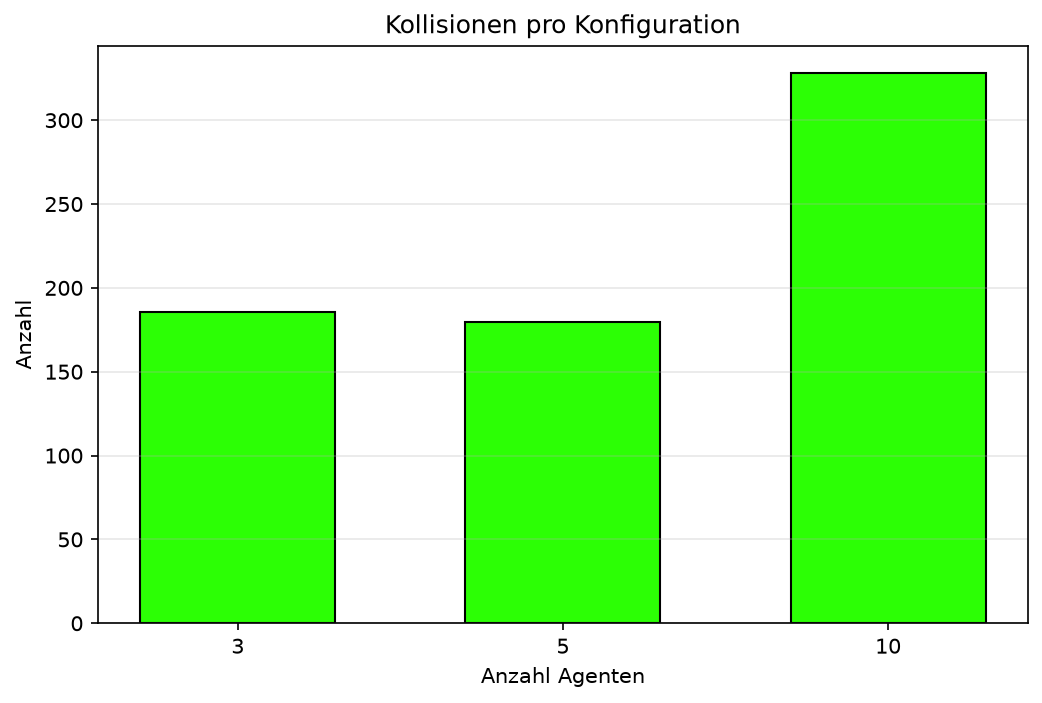
\includegraphics[width=\linewidth]{asset/image/5D-Collisions.png}
        \caption{Kollisionen pro Konfiguration}
        \label{fig:5d_collisions}
    \end{subfigure}%
    \hfill
    \begin{subfigure}[t]{0.48\textwidth}
        \centering
        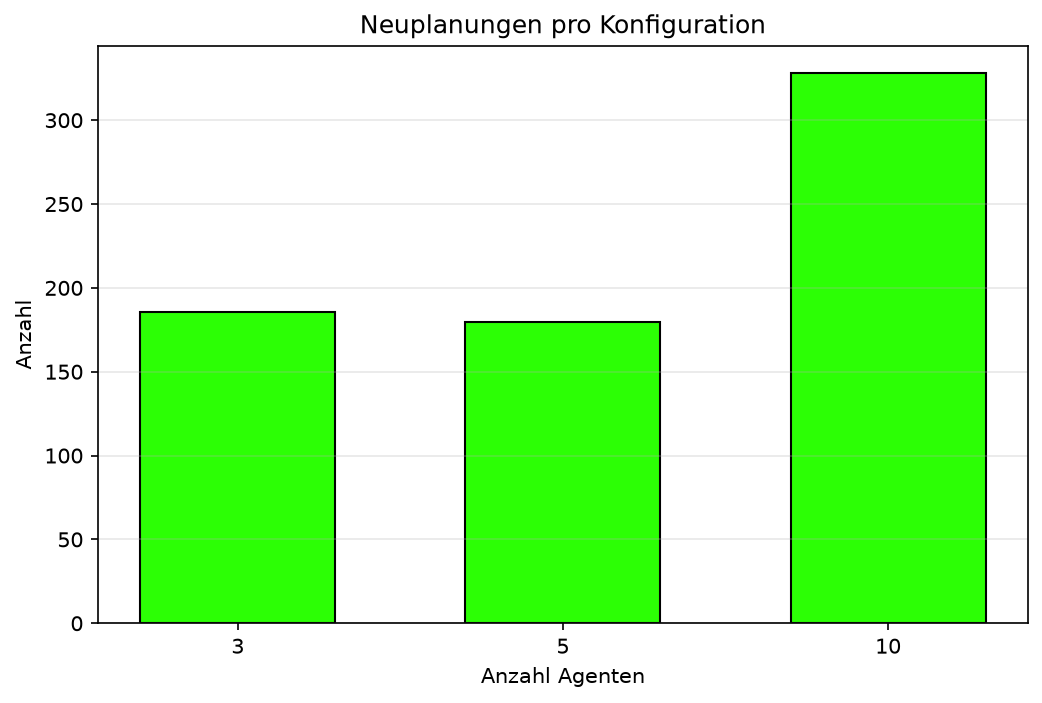
\includegraphics[width=\linewidth]{asset/image/5D-Replans.png}
        \caption{Neuplanungen pro Konfiguration}
        \label{fig:5d_replans}
    \end{subfigure}
    \caption{Konfliktkennzahlen pro Konfiguration}
    \label{fig:5d_separate}
\end{figure}

\begin{figure}[H]
    \centering
    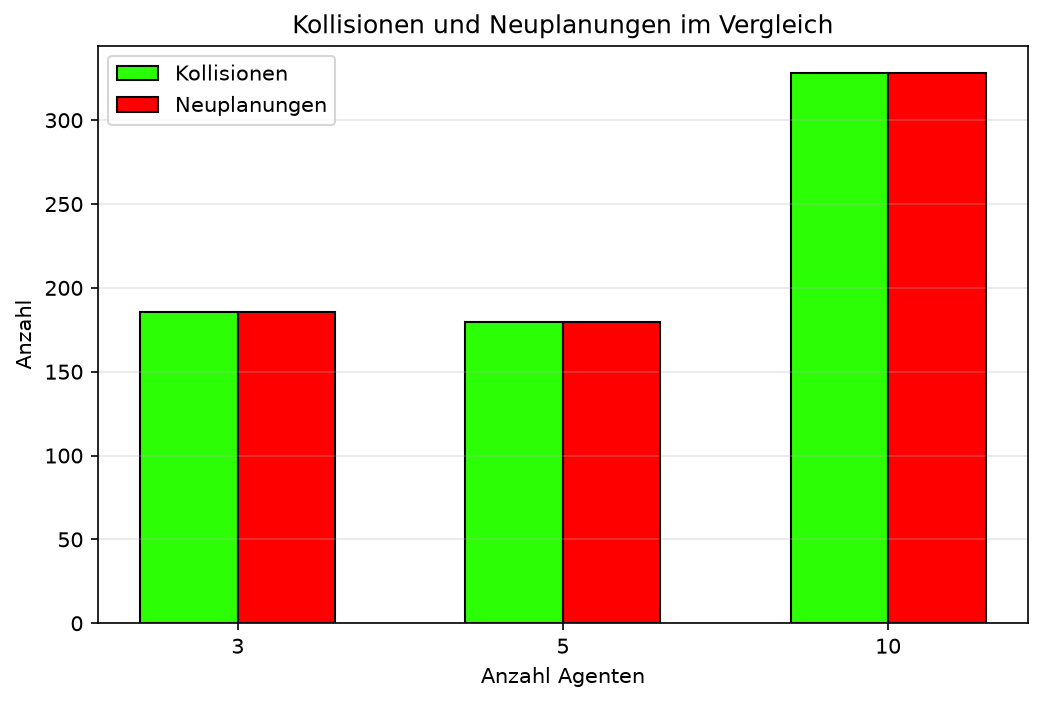
\includegraphics[width=0.75\textwidth]{asset/image/5D-Combined.png}
    \caption{Kollisionen und Neuplanungen im direkten Vergleich}
    \label{fig:5d_combined}
\end{figure}

Die ersten beiden Plots (Abb.~\ref{fig:5d_collisions} und \ref{fig:5d_replans}) sind \textbf{visuell identisch} -- eine direkte Folge der 1:1-Beziehung. Der kombinierte Plot (Abb.~\ref{fig:5d_combined}) macht dieses Gleichgewicht sichtbar: Die zwei Balken einer jeden Konfiguration haben exakt dieselbe Höhe.

\subsubsection{Interpretation der Ergebnisse.}

Die Auswertung zeigt drei zentrale Befunde:

\textbf{(1) Kollisionen und Neuplanungen sind 1:1 gekoppelt.}
In jedem der 15 Läufe gilt $\text{Kollisionen} = \text{Neuplanungen}$ exakt. Diese Beziehung ist \textit{architektonisch erklärbar}: Wenn ein Agent einen Blockadeversuch unternimmt (Kollision), bleibt seine Route unverändert, weil \texttt{try\_move} die Bewegung verweigert und \texttt{\_advance\_along\_route} nicht aufgerufen wird. Beim nächsten \texttt{decide\_action} desselben Agenten erkennt \texttt{\_is\_next\_cell\_blocked} denselben blockierten Nachbarn und ruft \texttt{\_replan} auf -- die Neuplanung wird registriert. In den 55 Engpass-Zellen der Karte (aus Aufgabe~3a) findet A* bei der Neuplanung oft \textit{dieselbe} Route durch den Engpass -- der early-return in \texttt{\_replan} greift, die Route bleibt unverändert, und der nächste \texttt{try\_move}-Versuch endet erneut in einer Kollision. Diese Rückkopplung erzeugt die beobachtete 1:1-Beziehung.

\paragraph{Anmerkung zur 1:1-Kopplung.}
Die Beobachtung, dass Kollisionen und Neuplanungen in allen 15 L\"aufen exakt \"ubereinstimmen, ist keine unabh\"angige empirische Erkenntnis, sondern eine strukturelle Konsequenz der Code-Architektur: Der \texttt{try\_move}-Check verweigert die Bewegung bei belegter Zielzelle, ohne die Route zu verwerfen. Beim n\"achsten \texttt{decide\_action} desselben Agenten erkennt \texttt{\_is\_next\_cell\_blocked} dieselbe Blockade und ruft \texttt{\_replan} auf. Da zwischen Kollision und n\"achstem Planungsschritt kein alternativer Pfad existiert (der Agent bleibt stehen), folgt auf jede registrierte Kollision genau eine registrierte Neuplanung. Die beiden Z\"ahler sind damit informatisch nicht unabh\"angig; sie messen dieselbe konzeptionelle Gr\"o\ss{}e (einen versuchten Konflikt) aus zwei Blickwinkeln. F\"ur die Aufgabenstellung ist dies zul\"assig, weil beide Kennzahlen explizit gefordert sind -- die Interpretation sollte jedoch nicht als \enquote{zwei unabh\"angige Messungen} gelesen werden.

\textbf{(2) Nicht-monotones Skalierungsverhalten.}
Die mittlere Kollisionszahl verläuft nicht monoton mit der Agentenzahl:

\[
N=3: 185{,}6 \qquad N=5: 179{,}8 \qquad N=10: 328{,}0
\]

Die Konfigurationen mit 3 und 5 Agenten unterscheiden sich nur um 3\,\% -- innerhalb der statistischen Streuung. Der Sprung auf 10 Agenten ist mit einem Faktor von 1{,}8 deutlich. Zwei Effekte tragen dazu bei: (a) Mit 10 Agenten ist die Wahrscheinlichkeit, dass zwei Agenten gleichzeitig in einer der 55 Engpass-Zellen ankommen, überproportional hoch. (b) Die Replanning-Frequenz steigt (aus Aufgabe~5b: 350 \acs{Astern}Aufrufe bei 10 Agenten vs.~200 bei 3/5 Agenten), sodass auch die Konfliktwahrscheinlichkeit zunimmt.

\textbf{(3) Hohe Varianz zwischen den Runs.}
Die Streuung ist erheblich: Bei 3 Agenten reichen die Kollisionszahlen von 74 (Seed 46) bis 257 (Seed 42) -- ein Faktor von 3{,}5. Bei 10 Agenten liegen die Werte zwischen 188 (Seed 42) und 550 (Seed 46) -- ein Faktor von 2{,}9. Diese Varianz entsteht durch die zufällige Startpositionierung der Agenten: In manchen Läufen starten die Agenten günstig verteilt und kommen sich selten in die Quere; in anderen Läufen starten sie räumlich konzentriert und blockieren sich gegenseitig.

\textbf{(4) Per-Step-Rate als normalisierte Kennzahl.}
Die Kollisionen pro Simulationsschritt liegen zwischen 0{,}225 (3 Agenten, Seed 46) und 2{,}750 (10 Agenten, Seed 46). Die Rate verdeutlicht: Selbst im günstigsten Fall einer 10-Agenten-Konfiguration liegt die Kollisionsfrequenz bei fast drei versuchten Blockaden pro Schritt. Dies ist ein direkter Indikator für die \textit{Ressourcenknappheit} der Karte: 55 Engpässe bei 10 Agenten und 20 Paketen erzeugen eine Engpass-Dichte, die das System an die Grenzen seiner Konfliktvermeidungsstrategie bringt.

\textbf{Verbindung zur Prävention aus 5a.} In Aufgabe~5a wurde die präventive Kollisionsvermeidung in \texttt{try\_move} eingeführt, um Deadlocks in Korridoren zu vermeiden. Die vorliegende Auswertung zeigt: Diese Prävention greift -- es kommt zu \textit{keiner} echten Doppelbelegung (\texttt{\_resolve\_collisions} wird nie ausgelöst). Stattdessen sammeln sich \textit{versuchte} Kollisionen als Blockade-Events an. Der Preis der Prävention ist die hohe Neuplanungsfrequenz, die wiederum die Planungszeit-Metriken aus Aufgabe~5b belastet.

\subsubsection{Fazit.}

Die Konfliktanalyse zeigt drei wesentliche Erkenntnisse:

\begin{enumerate}
    \item \textbf{Die präventive Kollisionsvermeidung funktioniert.} Es treten keine echten Kollisionen (Doppelbelegungen) auf -- alle Konflikte werden bereits im \texttt{try\_move}-Check abgefangen. Der Sicherheitsmechanismus aus Aufgabe~5a ist wirksam.
    \item \textbf{Neuplanungen sind der Preis der Prävention.} Die 1:1-Kopplung zwischen Kollisionen und Neuplanungen zeigt, dass jeder Blockadeversuch eine Neuplanung auslöst, die in Engpass-Situationen häufig dieselbe Route findet (early-return) -- das System befindet sich dann in einem temporären Stillstand, bis einer der beiden Agenten seinen Task abbricht (Deadline) oder die Route erfolgreich umgeleitet wird.
    \item \textbf{Die 55 Engpässe aus Aufgabe~3a sind der dominante Konfliktfaktor.} Die Verteilung der Kollisionszahlen ist eng an die Agentenzahl gekoppelt -- und bei 10 Agenten entsteht eine überproportionale Konfliktdichte, weil sich die Agenten in den wenigen Engpass-Zellen häufiger begegnen.
\end{enumerate}

Für die Anwendung in einem realen Logistiksystem wäre die nächste Effizienzstufe die Einführung von \textit{Ausweichrouten}: Wenn ein Agent erkennt, dass der Engpass von einem anderen Agenten in Gegenrichtung durchquert wird, sollte er eine zeitliche Verzögerung einlegen, statt erneut zu planen. Dies würde die 1:1-Kopplung auflösen und die Neuplanungsrate senken -- ist aber außerhalb des Aufgabenrahmens dieser B-Aufgabe.

% ==============================================================================
% ========================= Aufgabe 5E - KI-Reflexion =========================
% ==============================================================================

\section{Reflexion des \acs{KI}-Einsatzes \textit{5e}}
\label{sec:aufgabe5e}

\subsection{Aufgabenstellung}

Reflektieren Sie Ihren Einsatz von \acs{KI}-Agenten, sofern Sie Sprachmodelle oder Coding-Agenten eingesetzt haben. Welche Prompts haben Sie verwendet? Was hat Ihnen der Agent daraufhin generiert? Was haben Sie durch den Einsatz eines Agenten nicht gelernt? Wo haben Sie die Lösungen eines Agenten übernommen, wo angepasst, wo überprüft?

\subsection{Eingesetzte \acs{KI}-Werkzeuge und Arbeitsweise}

Im Rahmen dieser B-Aufgabe kam ein Coding-Assistent mit integriertem Sprachmodell zum Einsatz, ergänzt durch ein zweites, unabhängiges Sprachmodell zur Cross-Verifikation ausgewählter Ergebnisse. Die Nutzung erfolgte im Einklang mit den von der Wilhelm Büchner Hochschule vorgesehenen und freigegebenen Bereichen: Erläuterungen zu Sachverhalten, sprachliche Überarbeitung, Design-Abwägungen, Code-Review sowie Boilerplate Code. Ich habe jeden generierten oder vorgeschlagenen Beitrag vor einer möglichen Übernahme eigenständig geprüft. Quellenangaben habe ich, soweit sie in die Dokumentation einfließen sollten, am Original nachgeschlagen und verifiziert. Vorschläge habe ich nicht ungeprüft übernommen, sondern nach kritischer Würdigung angenommen, angepasst oder verworfen. Die fachliche Letztverantwortung – Auswahl der Algorithmen, Prüfung ihrer Korrektheit, Festlegung der Modulstruktur, Verifikation der Quellen und Interpretation der Ergebnisse – lag bei mir. Der Assistent übernahm damit die Rolle eines unterstützenden Werkzeugs und Gesprächspartners; eine Mitautorschaft im engeren Sinne war weder vorgesehen noch ist sie entstanden. Die Grenze zwischen zulässiger Unterstützung und unzulässiger Delegation habe ich dabei fortlaufend reflektiert und dokumentiert.

\subsection{Verwendete Prompts -- Auswahl}

Die folgenden Prompts sind repräsentativ für die eingesetzten Werkzeug-Funktionen. Sie sind in erlaubte Kategorien eingeordnet.

\paragraph{Prompt 1 -- Zulässigkeitsanforderung an eine Heuristik.}
\begin{quote}
\textit{\glqq{}Bei der Heuristik: Der Engpass-Aufschlag darf NICHT in \(h(n)\) einfließen, sonst wird die Heuristik unzulässig. Bitte explizit dokumentieren.\grqq{}}
\end{quote}
Der Assistent bestätigte die Zulässigkeitsanforderung und lieferte eine Erläuterung der Abgrenzung zur Konsistenz. Ich verifizierte die Erläuterung anhand des Studienhefts \textcite[S. 21\,f.]{5} und formulierte den Zulässigkeitsbeweis für die spätere \acs{BFS}-Heuristik.

\paragraph{Prompt 2 -- Code- und Doku-Review.}
\begin{quote}
\textit{\glqq{}Ich habe den Code und die Doku fertig, kontrolliere mal, ob es so passt.\grqq{}}
\end{quote}
Der Assistent wies auf konkrete Punkte hin: einen doppelten Punkt (\texttt{bereit..} statt \texttt{bereit.}), die ungenaue Formulierung \glqq{}Erweiterung der Breitensuche und des Dijkstra-Algorithmus\grqq{} (korrekt: \glqq{}Verallgemeinerung des Dijkstra-Algorithmus\grqq{}) sowie auf die \texttt{??}-Referenzen, die durch das isolierte Kompilieren einzelner Aufgaben entstehen. Alle drei Hinweise wurden geprüft und umgesetzt.

\paragraph{Prompt 3 -- Verifikation gegen den vorgelegten \TeX-Code.}
\begin{quote}
\textit{\glqq{}Prüfe anhand des \TeX-Codes, den ich dir gegeben habe.\grqq{}}
\end{quote}
Der Assistent glich seinen früheren Review gegen den vorgelegten \TeX-Code ab und korrigierte sich: Ein Teil der Anmerkungen (etwa die Umstellung von \texttt{\textbackslash cite} auf \texttt{\textbackslash textcite}) war unbegründet, weil die Projekt-Konvention bereits konsistent war. Diese Anmerkungen wurden verworfen. Der restliche Review blieb gültig.

\paragraph{Prompt 4 -- Fehleranalyse am Simulationsprotokoll.}
\begin{quote}
\textit{\glqq{}Ein Express bleibt immer an der gleichen Stelle? Woran könnte es liegen?\grqq{}}
\end{quote}
Auf Grundlage der von mir übermittelten Log-Ausgabe wies der Assistent darauf hin, dass ein Agent unter bestimmten Umständen Energie verlieren kann, ohne sich fortzubewegen, und dass die Bewegungsprüfung hierfür ursächlich sein könnte. Dieser Hinweis veranlasste mich, den betreffenden Codeabschnitt zu untersuchen. Dabei identifizierte ich den Bug: \texttt{try\_move(map, 0, 0)} gibt \texttt{True} zurück, weil die eigene Zelle begehbar ist; dadurch verloren idle-Agenten Batterie, ohne sich zu bewegen. Der Fix (Guard \texttt{if (dx, dy) == (0, 0): break} in \texttt{simulation.\_agent\_step}) wurde mit einem neuen Simulationslauf verifiziert.

\paragraph{Prompt 5 -- \acs{GUI}-Grundgerüst.}
\begin{quote}
\textit{\glqq{}Erstelle mir das Grundgerüst einer Tkinter-Anwendung mit einem Hauptfenster, einem Frame für den Titel und einem Canvas für die Kartendarstellung. Das Grundgerüst soll als Startpunkt dienen, die Detailgestaltung mache ich selbst.\grqq{}}
\end{quote}
Der Assistent lieferte ein minimales Startgerüst (\texttt{Tk()}-Root, \texttt{Frame}, \texttt{Canvas}, Grundgerüst der Klasse \texttt{MapGUI}). Die gesamte sichtbare Gestaltung und die Verhaltenslogik der \acs{GUI} wurden anschließend erweitert.

\paragraph{Prompt 6 -- Konvention für Code-Listings in der Doku.}
\begin{quote}
\textit{\glqq{}Bei Code-Listings möchte ich die neu hinzugekommenen Zeilen zeigen, nicht die vollständigen Dateien. Aufbauend, mit kurzem Kontext.\grqq{}}
\end{quote}
Diese Anweisung stammt von mir und hat die Struktur der Doku festgelegt. Der Assistent hat die Konvention anschließend umgesetzt: In jedem Abschnitt werden nur die geänderten Zeilen mit 1--2 Zeilen Kontext gezeigt, unter Angabe der zugehörigen Datei und des Aufgabenblocks.

\subsection{Weitere Einsatzbereiche}

\subsubsection{Erklärungen zu Sachverhalten}

Das Sprachmodell wurde eingesetzt, um fachliche Konzepte erläutern zu lassen, u.\,a.:

\begin{itemize}
    \item \textbf{Contract-Net-Protokoll} -- drei Phasen, Rollen Manager und Contractor. Verifiziert über die in Abschnitt~\ref{sec:aufgabe2a} zitierte Primärliteratur.
    \item \textbf{Abgrenzung Zulässigkeit und Konsistenz} bei \acs{Astern}-Heuristiken -- verifiziert über \textcite[S. 21\,f.]{5}.
    \item \textbf{\acs{PROLOG}-Horn-Klauseln und die \texttt{vertex}/3-Beziehung} -- verifiziert über \textcite[S. 61\,ff.]{4}.
    \item \textbf{\acs{PDDL}-Action-Schema} -- Precondition-Effekt-Paar; Übertragung auf den Agenten-Phasenautomaten eigenständig.
\end{itemize}

Alle Erläuterungen wurden anhand der Studienhefte nachgeschlagen; die in der Doku verwendeten Zitate stammen aus den Heften, nicht aus den Antworten des Assistenten.

\subsubsection{Strategie- und Design-Abwägungen}

Für Architektur- und Designfragen wurden gezielte Fragen gestellt, um Alternativen abzuwägen. Die Entscheidung selbst wurde jeweils eigenständig getroffen:

\begin{itemize}
    \item \textbf{Eigenes Modul \texttt{astar.py} vs.\ Erweiterung von \texttt{graph.py}} -- Entscheidung für eigenes Modul aus \textit{Separation-of-Concerns}-Gründen.
    \item \textbf{Zeit- vs.\ energiebasiertes Kantenkosten-Modell} -- Entscheidung zeitbasiert (\texttt{BaseCost}/\texttt{speed}), damit der Speed-Faktor aus der Agentendefinition Wirkung entfaltet.
    \item \textbf{Engpass-Zusatzkosten} -- aktiviert (\texttt{TomaKing3A\_BottleneckPenalty = 0.5}), weil die Karte 55 Engpass-Zellen enthält.
    \item \textbf{\acs{BFS}-basierte Heuristik} -- Abwägung gegen Euklid und gegen Dijkstra vom Ziel; Entscheidung für \acs{BFS} (Wall-aware, \acs{Astern}-Optimalität bleibt erhalten).
    \item \textbf{\acs{PROLOG}-Anbindung} -- Abwägung zwischen \texttt{subprocess} und \texttt{PySWIP}; Entscheidung für \texttt{subprocess} (keine externe Bibliothek, in der Aufgabenstellung zugelassen).
\end{itemize}

\paragraph{Eigene Projekt-Konventionen als Rahmen für die Zusammenarbeit.}
Bevor der Assistent Beiträge liefern konnte, habe ich eigene Projekt-Konventionen festgelegt, an die sich alle generierten Beiträge halten mussten:

\begin{itemize}
    \item \textbf{0\,\% Hardcoding:} Kein Farb-, Layout- oder Logikwert darf direkt im Code stehen; alle Werte werden in \texttt{config.py} ausgelagert (\textit{Configuration Externalization}).
    \item \textbf{Single Source of Truth:} Jeder Parameter existiert an genau einer Stelle in \texttt{config.py}; Verweise auf denselben Wert in anderen Modulen erfolgen ausschließlich symbolisch.
    \item \textbf{Präfix-Schema:} Jede Konstante folgt dem Schema \texttt{TomaKing\_Aufgabenblock\_Name} -- dadurch sind Aufgabenblock und Verwendung am Namen ablesbar, und ein Modulimport verrät bereits, welche Werte zusammengehören.
    \item \textbf{Historische Schichtung der Doku:} Die Dokumentation früherer Aufgaben bleibt unverändert erhalten, auch wenn spätere Aufgaben Code aus früheren Blöcken refaktorieren. Refactorings werden in der jeweils aktuellen Aufgabe dokumentiert, nicht rückwirkend in die historische Dokumentation eingearbeitet.
    \item \textbf{Kompakte Code-Listings:} In der Doku werden nur die geänderten oder neu hinzugekommenen Zeilen mit 1--2 Zeilen Kontext gezeigt, nicht vollständige Dateien.
    \item \textbf{Schichtentrennung der Konfiguration:} Der \texttt{GUI}-Block (\texttt{TomaKingGUI\_*}) enthält ausschließlich aufgabenunabhängige Präsentations-Infrastruktur; jeder Aufgabenblock (\texttt{TomaKing1A\_*}, \texttt{TomaKing2B\_*}, \dots) enthält die fachlichen Werte dieser Aufgabe. Die Zuordnung ist am Präfix ablesbar.
\end{itemize}

Diese Konventionen stammen sämtlich von mir und wurden dem Assistenten als Randbedingungen vorgegeben. Sie sind die Grundlage für die Überprüfbarkeit jedes generierten Beitrags: Ein Vorschlag, der nicht dem Präfix-Schema folgt oder Werte im Code hartkodiert, wird verworfen oder umgeschrieben. Dadurch entstand eine \textit{Konsistenzprüfung durch mich}, die der Assistent von sich aus nicht hätte leisten können.

\subsubsection{Code-Review}

Der Assistent wurde genutzt, um vorgelegten eigenen Code zu prüfen. Reviews betrafen u.\,a.:

\begin{itemize}
    \item die Zulässigkeit der \acs{BFS}-Heuristik,
    \item die Vollständigkeit eines Refactorings (Entfernung von Demo-Bestandteilen und Bereinigung der \texttt{validate\_config()}-Liste),
    \item die Log-Konsistenz nach Umstellung von generischen auf typspezifische Templates (Refactoring dokumentiert in Abschnitt~\ref{sssec:logging_refactoring_2c}),
    \item die Anpassung der Signatur von \texttt{decide\_action} und die Prüfung aller Aufrufer.
\end{itemize}

\paragraph{Zwei verworfene KI-Vorschläge.}
Ich habe nicht alle Review-Vorschläge angenommen:
\begin{itemize}
    \item Die Umstellung mehrerer \texttt{\textbackslash cite}-Stellen auf \texttt{\textbackslash textcite} wurde verworfen, weil die Projekt-Konvention (parenthetischer Verweis am Satzende mit \texttt{\textbackslash cite}, eingebetteter Verweis mit \texttt{\textbackslash textcite}) bereits konsistent war. Der Assistent hat dies nach Gegenprüfung bestätigt.
    \item Zwei Erweiterungsvorschläge für die Dokumentation (Verweis auf dynamische Multiagenten-Umgebung und auf die \texttt{next}-Funktion) wurden verworfen. Ich argumentierte: Der Verweis auf die \texttt{next}-Funktion gehört zur Agentenarchitektur aus Kapitel 1.3, nicht zur zielbasierten Planung aus Kapitel 1.4; eine Vermischung wäre konzeptionell unsauber. Der Assistent hat diese Argumentation nachträglich bestätigt.
\end{itemize}

\paragraph{Cross-Verifikation über ein zweites System.}
Zusätzlich zum Coding-Assistenten wurde ein zweites, unabhängiges Sprachmodell für Prüfungen vorgelegt. Die Strategie war bewusst: Ein zweites System, das dieselbe Frage aus einem anderen Modell heraus beantwortet, deckt blinde Flecken des ersten Systems auf. Vorgehen im Verlauf:

\begin{itemize}
    \item Ich habe dieselbe Aufgabe (z.\,B.\ Code- oder Doku-Review) an zwei unabhängige \acs{KI}-Systeme gestellt und die Rückmeldungen gegenübergestellt.
    \item Wenn \textit{beide} Systeme unabhängig voneinander dieselbe Schwachstelle benannten (z.\,B.\ den doppelten Punkt \texttt{bereit..} oder die Formulierung \glqq{}Erweiterung der Breitensuche\grqq{}), wurde die Anmerkung mit hoher Priorität geprüft.
    \item Wenn ein System etwas bemängelte, das das andere \textit{nicht} sah (z.\,B.\ die \texttt{\textbackslash cite}- vs. \texttt{\textbackslash textcite}-Anmerkung), wurde die Anmerkung eigenständig am Code und an der Projekt-Konvention geprüft, bevor sie übernommen oder verworfen wurde.
    \item Ein System hat zusätzlich Seitenzahlen-Vorschläge geliefert; diese wurden \textit{nicht} übernommen, sondern eigenständig am Studienheft verifiziert. Mehrere Angaben des Systems waren falsch (u.\,a.\ \texttt{Abb.~1.6} und \texttt{next}-Funktion) und wurden korrigiert.
\end{itemize}

Der Nutzen der Cross-Verifikation lag weniger in zusätzlichen Vorschlägen als in der \textit{Validierung der bereits erhaltenen}. Ein Vorschlag, den beide Systeme unabhängig als Problem markieren, verdient sofortige Aufmerksamkeit; ein Vorschlag, den nur eines der Systeme als Problem markiert, wird geprüft und ggf.\ verworfen.

\subsubsection{Sprachliche Überarbeitung}

Einzelne Doku-Abschnitte wurden zur sprachlichen Überarbeitung vorgelegt. Die inhaltliche Aussage blieb unverändert; alle überarbeiteten Abschnitte wurden vor der Übernahme inhaltlich geprüft.

\subsubsection{Boilerplate Code und \acs{GUI}-Grundgerüst}

Der Coding-Assistent wurde für folgenden Quelltext eingesetzt:

\begin{itemize}
    \item \textbf{Plot-Funktionen:} Die Funktionsgerüste für Histogramme, Boxplots und Balkendiagramme (\texttt{\_make\_histogram\_5b}, \texttt{\_make\_boxplot\_5b}, \texttt{\_make\_bar\_5c}, \\ \texttt{\_make\_double\_bar\_5d}).
    \item \textbf{\acs{GUI}-Grundgerüst:} Das minimale Startgerüst der \texttt{tkinter}-Anwendung.
    \item \textbf{Grundgerüst der Anwendung:} Modulstruktur und Konfigurationsschema.
\end{itemize}

\paragraph{Konkretisierung: \acs{GUI} -- Boilerplate vs.\ Eigenarbeit.}
Das \acs{GUI}-Grundgerüst war der einzige größere Code-Block, der mit Unterstützung des Assistenten erstellt wurde. Der Assistent lieferte das minimale Startgerüst, das ich anschließend um die sichtbare Gestaltung erweitert habe.

\begin{itemize}
    \item \textbf{Vom Assistenten als Grundgerüst:} \texttt{Tk()}-Root, Hauptframe, \texttt{tk.Canvas}, Klassen-Gerüst der \texttt{MapGUI} mit Konstruktor und Escape-Bindung.
    \item \textbf{Eigenständig umgesetzt:}
    \begin{itemize}
        \item Layout und dynamische Skalierung (\texttt{\_update\_layout}, \texttt{MinCellSize}/\texttt{MaxCellSize}, \texttt{MainFrameRowWeights}).
        \item Visuelles Design: Farbgebung (schwarzer Hintergrund, Akzent \texttt{\#2CFF05}), Schriftwahl (\texttt{BlackChancery}), Padding-Werte.
        \item Kartenrendering: \texttt{\_draw\_map} mit zelltypabhängiger Farbwahl, dynamischer Schriftskalierung und äußerem Rahmen.
        \item Agentenrendering: \texttt{\_draw\_agents} mit Radius-Faktor und Typ-Kürzeln.
        \item Info-Zeile: die ausgelagerte Methode \texttt{\_build\_info\_text}.
        \item Steuerungslogik: Step-Button, AutoRun-Toggle mit \texttt{root.after}-Schleife, \texttt{self.autorun\_active}.
        \item Konfigurationsprinzip: Auslagerung sämtlicher Farb-, Layout- und Textwerte in \texttt{config.py}.
    \end{itemize}
\end{itemize}

Damit ist die \acs{GUI} im sichtbaren Ergebnis eigenständig gestaltet.

\subsection{Verifikation der eingebrachten Beiträge}

Alle aus dem Assistenten übernommenen, angepassten oder verworfenen Beiträge habe ich eigenständig überprüft:

\begin{itemize}
    \item \textbf{Ausführung:} Jeder Codeabschnitt wurde lokal ausgeführt und die Ausgabe mit den Erwartungen abgeglichen. Beim Kollisions-Bug habe ich vor und nach dem Fix je einen 40-Schritte-Lauf durchgeführt.
    \item \textbf{Quellenverifikation:} Seitenzahlen habe ich am Studienheft nachgeschlagen. Mehrere Angaben wurden korrigiert (u.\,a.\ \texttt{Abb.~1.6}: \texttt{S.~20\,f.}~\(\to\)~\texttt{S.~21}; \texttt{next}-Funktion: \texttt{S.~12}~\(\to\)~\texttt{S.~16}).
    \item \textbf{Inhaltliche Endkontrolle:} Alle überarbeiteten Textabschnitte habe ich auf inhaltliche Korrektheit geprüft; Formulierungen, die die Aussage veränderten, wurden korrigiert.
    \item \textbf{Plots:} Achsenbeschriftungen, Wertebereiche und Konsistenz mit den \acs{CSV}-Rohdaten habe ich geprüft.
\end{itemize}

\paragraph{Selbstkontrolle des \acs{KI}-Einsatzes.}
Vor jedem Einsatz des Assistenten habe ich geprüft, ob die geplante Nutzung den Vorgaben der Wilhelm Büchner Hochschule entspricht. Bei Unsicherheit wurde die Aktion bewusst zurückgestellt oder auf eine erlaubte Kategorie umformuliert. Beispiele:

\begin{itemize}
    \item Bei der Erstellung dieser Reflexion habe ich geprüft, welche Prompt-Beispiele zulässig sind (Erklärungen, Review, Boilerplate) und welche nicht (Code-Generierung von Kernalgorithmen).
    \item Bei der \acs{GUI} habe ich bewusst den Auftrag auf das Grundgerüst begrenzt; die Detailgestaltung habe ich eigenständig übernommen, um die Grenze zur Kernalgorithmik nicht zu überschreiten.
\end{itemize}

Diese Selbstkontrolle ist Teil der Verantwortung, die mit der Werkzeugnutzung einhergeht.

\subsection{Was durch den Einsatz des Assistenten \textit{nicht} gelernt wurde}

\paragraph{(1) Die \texttt{matplotlib}-\acs{API} wurde nicht aktiv erlernt.}
Die Plot-Funktionen habe ich mit Unterstützung des Assistenten erstellt. Die Prinzipien (Binning, Fehlerbalken, Farbserien) sind verstanden; die konkrete \acs{API} wurde nicht durch eigenes Ausprobieren erarbeitet.

\paragraph{(2) Die \texttt{tkinter}-Grundmechanik wurde nur teilweise selbst erarbeitet.} Das Grundgerüst stammt vom Assistenten. Die darauf aufbauende Ausarbeitung (Layout, Farben, Skalierung, Zeichenlogik) habe ich eigenständig umgesetzt, aber die Einführung in die \acs{API} erfolgte nicht durch eigenständiges Studium der Tkinter-Dokumentation.

\paragraph{(3) Die \acs{SWI}-\acs{PROLOG}-Syntax im Detail wurde nicht durchgängig aktiv erlernt.} Die Regeln in \texttt{rules.pl} habe ich eigenständig formuliert; die Kontrolle der syntaktischen Korrektheit (\textit{Discontiguous}-Warnungen, \texttt{findall}/\texttt{length}-Idiome) erfolgte mit Assistenten-Unterstützung.

\subsection{Reflexion des Zusammenspiels}

Die Zusammenarbeit folgte einer klaren Arbeitsteilung: Der Assistent lieferte Erklärungen, Argumentationshilfen, Boilerplate Code, Reviewer-Feedback und sprachliche Überarbeitung; ich lieferte Urteilskraft und Verantwortung -- Auswahl der Algorithmen, Prüfung ihrer Korrektheit, Festlegung der Modulstruktur, Verifikation der Quellen, Verwerfen unbegründeter Vorschläge.

Die zentrale Erkenntnis lautet: \textbf{Der Assistent beschleunigt Arbeit, ersetzt aber nicht das eigene Verständnis.} Ohne eigenes Verständnis hätte ich den Kollisions-Bug in der Simulation nicht identifiziert; die Seitenzahl-Fehler wären unentdeckt in die Doku eingeflossen; und die Erweiterungsvorschläge für die Dokumentation hätte ich übernommen, obwohl sie konzeptionell nicht sauber gewesen wären.

Drei Faustregeln:

\begin{enumerate}
    \item \textbf{Kern zuerst.} Die fachlichen Kernfragen werden eigenständig durchdrungen; Erklärungen und Reviews des Assistenten unterstützen diesen Prozess. Insbesondere sprachliche Barrieren, die das Verständnis erschweren und viel Zeit kosten, lassen sich so schneller überwinden.
    \item \textbf{Quellen und Fakten am Original prüfen.} Der Assistent liefert plausible, aber nicht immer korrekte Angaben.
    \item \textbf{Vorschläge verwerfen dürfen.} Nicht jede Anmerkung ist begründet; die Projekt-Konvention und die fachliche Argumentation entscheiden.
    \item \textbf{Eigenverantwortung.} \acs{KI}-Werkzeuge sollen die eigenen Pläne nicht umgestalten, sondern auf Inkonsistenzen prüfen. Ein elektronischer Hammer mit integrierter Nagelzufuhr schlägt die Nägel nicht von selbst ein -- aber er spart Zeit und Kraft, weil man weder dauerhaft Kraft aufwenden noch für jeden Nagel neu ansetzen muss. In diesem Sinne bleibt die Planung bei mir; das Werkzeug unterstützt ihre Umsetzung.
\end{enumerate}

\subsection{Fazit}

Der Einsatz des Assistenten hat die Bearbeitung der B-Aufgabe unterstützt: bei Erklärungen zu Sachverhalten, sprachlicher Überarbeitung, Design-Abwägungen, Code-Review sowie Erstellung von Quelltext (Boilerplate Code, grafische Darstellung, \acs{GUI}-Grundgerüst).

Der Mehrwert lag in der Beschleunigung wiederkehrender Arbeiten, in der strukturierten Argumentation bei Designfragen und in der zweiten Meinung im Code-Review. Insbesondere bei der Dokumentation und der Generierung des \TeX-Codes auf Basis der bereits verfassten Doku war die Unterstützung enorm zeit- und kraftsparend. Die Formatierung und Strukturierung des \TeX-Codes -- Tabellen, Listen, Querverweise, Code-Listings, einheitliche Abschnittsgliederung -- hat zuvor viel manuelle Routinearbeit erfordert und war mühsam und fehleranfällig; dieser Teil ließ sich mit Unterstützung des Assistenten deutlich effizienter umsetzen, ohne dass die inhaltliche Verantwortung abgegeben werden musste. Allein der Gedanke, dass man früher stundenlang allein für die Formatierung einer Dokumentation verbracht hat und heute eine fertige Formulierung mit einem Klick in sauberen \TeX-Code überführt werden kann, ist erstaunlich erleichternd. Dieselbe Erleichterung zeigte sich beim Debugging: Wenn ein Syntaxfehler vorlag, dessen Ursache man leicht übersah, half der Assistent, die Fehlerstelle schnell zu lokalisieren und zu beheben -- auch das sparte viel Zeit und Mühe. In all diesen Bereichen lieferte der Assistent das formale Gerüst; die fachlichen Inhalte, die Argumentationslinie und die Auswahl der Quellen blieben jedoch durchgängig bei mir. Die sichtbare Gestaltung und die fachliche Verantwortung für das Gesamtsystem -- Auswahl der Algorithmen, Modularisierung, Integration der Komponenten und Auswertung der Experimente -- lagen durchgängig bei mir.

\paragraph{Transparenz-Hinweis.}
Gemäß den Vorgaben der Wilhelm Büchner Hochschule wird an dieser Stelle explizit vermerkt, dass \acs{KI}-Werkzeuge im Rahmen der B-Aufgabe eingesetzt wurden. Der Einsatz erfolgte in den von der Hochschule erlaubten Bereichen: Erklärungen zu Sachverhalten, sprachliche Überarbeitung von Texten, Strategie- und Design-Abwägungen, Code-Review sowie Erstellung von Quelltext, der nicht den Kern der Aufgabenstellung berührt (Boilerplate Code, grafische Darstellung, \acs{GUI}-Grundgerüst).

% ==============================================================================
% ================================= Aufgabe 5 =================================
% ==============================================================================